% Options for packages loaded elsewhere
\PassOptionsToPackage{unicode}{hyperref}
\PassOptionsToPackage{hyphens}{url}
%
\documentclass[
]{book}
\usepackage{amsmath,amssymb}
\usepackage{iftex}
\ifPDFTeX
  \usepackage[T1]{fontenc}
  \usepackage[utf8]{inputenc}
  \usepackage{textcomp} % provide euro and other symbols
\else % if luatex or xetex
  \usepackage{unicode-math} % this also loads fontspec
  \defaultfontfeatures{Scale=MatchLowercase}
  \defaultfontfeatures[\rmfamily]{Ligatures=TeX,Scale=1}
\fi
\usepackage{lmodern}
\ifPDFTeX\else
  % xetex/luatex font selection
\fi
% Use upquote if available, for straight quotes in verbatim environments
\IfFileExists{upquote.sty}{\usepackage{upquote}}{}
\IfFileExists{microtype.sty}{% use microtype if available
  \usepackage[]{microtype}
  \UseMicrotypeSet[protrusion]{basicmath} % disable protrusion for tt fonts
}{}
\makeatletter
\@ifundefined{KOMAClassName}{% if non-KOMA class
  \IfFileExists{parskip.sty}{%
    \usepackage{parskip}
  }{% else
    \setlength{\parindent}{0pt}
    \setlength{\parskip}{6pt plus 2pt minus 1pt}}
}{% if KOMA class
  \KOMAoptions{parskip=half}}
\makeatother
\usepackage{xcolor}
\usepackage{color}
\usepackage{fancyvrb}
\newcommand{\VerbBar}{|}
\newcommand{\VERB}{\Verb[commandchars=\\\{\}]}
\DefineVerbatimEnvironment{Highlighting}{Verbatim}{commandchars=\\\{\}}
% Add ',fontsize=\small' for more characters per line
\usepackage{framed}
\definecolor{shadecolor}{RGB}{248,248,248}
\newenvironment{Shaded}{\begin{snugshade}}{\end{snugshade}}
\newcommand{\AlertTok}[1]{\textcolor[rgb]{0.94,0.16,0.16}{#1}}
\newcommand{\AnnotationTok}[1]{\textcolor[rgb]{0.56,0.35,0.01}{\textbf{\textit{#1}}}}
\newcommand{\AttributeTok}[1]{\textcolor[rgb]{0.13,0.29,0.53}{#1}}
\newcommand{\BaseNTok}[1]{\textcolor[rgb]{0.00,0.00,0.81}{#1}}
\newcommand{\BuiltInTok}[1]{#1}
\newcommand{\CharTok}[1]{\textcolor[rgb]{0.31,0.60,0.02}{#1}}
\newcommand{\CommentTok}[1]{\textcolor[rgb]{0.56,0.35,0.01}{\textit{#1}}}
\newcommand{\CommentVarTok}[1]{\textcolor[rgb]{0.56,0.35,0.01}{\textbf{\textit{#1}}}}
\newcommand{\ConstantTok}[1]{\textcolor[rgb]{0.56,0.35,0.01}{#1}}
\newcommand{\ControlFlowTok}[1]{\textcolor[rgb]{0.13,0.29,0.53}{\textbf{#1}}}
\newcommand{\DataTypeTok}[1]{\textcolor[rgb]{0.13,0.29,0.53}{#1}}
\newcommand{\DecValTok}[1]{\textcolor[rgb]{0.00,0.00,0.81}{#1}}
\newcommand{\DocumentationTok}[1]{\textcolor[rgb]{0.56,0.35,0.01}{\textbf{\textit{#1}}}}
\newcommand{\ErrorTok}[1]{\textcolor[rgb]{0.64,0.00,0.00}{\textbf{#1}}}
\newcommand{\ExtensionTok}[1]{#1}
\newcommand{\FloatTok}[1]{\textcolor[rgb]{0.00,0.00,0.81}{#1}}
\newcommand{\FunctionTok}[1]{\textcolor[rgb]{0.13,0.29,0.53}{\textbf{#1}}}
\newcommand{\ImportTok}[1]{#1}
\newcommand{\InformationTok}[1]{\textcolor[rgb]{0.56,0.35,0.01}{\textbf{\textit{#1}}}}
\newcommand{\KeywordTok}[1]{\textcolor[rgb]{0.13,0.29,0.53}{\textbf{#1}}}
\newcommand{\NormalTok}[1]{#1}
\newcommand{\OperatorTok}[1]{\textcolor[rgb]{0.81,0.36,0.00}{\textbf{#1}}}
\newcommand{\OtherTok}[1]{\textcolor[rgb]{0.56,0.35,0.01}{#1}}
\newcommand{\PreprocessorTok}[1]{\textcolor[rgb]{0.56,0.35,0.01}{\textit{#1}}}
\newcommand{\RegionMarkerTok}[1]{#1}
\newcommand{\SpecialCharTok}[1]{\textcolor[rgb]{0.81,0.36,0.00}{\textbf{#1}}}
\newcommand{\SpecialStringTok}[1]{\textcolor[rgb]{0.31,0.60,0.02}{#1}}
\newcommand{\StringTok}[1]{\textcolor[rgb]{0.31,0.60,0.02}{#1}}
\newcommand{\VariableTok}[1]{\textcolor[rgb]{0.00,0.00,0.00}{#1}}
\newcommand{\VerbatimStringTok}[1]{\textcolor[rgb]{0.31,0.60,0.02}{#1}}
\newcommand{\WarningTok}[1]{\textcolor[rgb]{0.56,0.35,0.01}{\textbf{\textit{#1}}}}
\usepackage{longtable,booktabs,array}
\usepackage{calc} % for calculating minipage widths
% Correct order of tables after \paragraph or \subparagraph
\usepackage{etoolbox}
\makeatletter
\patchcmd\longtable{\par}{\if@noskipsec\mbox{}\fi\par}{}{}
\makeatother
% Allow footnotes in longtable head/foot
\IfFileExists{footnotehyper.sty}{\usepackage{footnotehyper}}{\usepackage{footnote}}
\makesavenoteenv{longtable}
\usepackage{graphicx}
\makeatletter
\def\maxwidth{\ifdim\Gin@nat@width>\linewidth\linewidth\else\Gin@nat@width\fi}
\def\maxheight{\ifdim\Gin@nat@height>\textheight\textheight\else\Gin@nat@height\fi}
\makeatother
% Scale images if necessary, so that they will not overflow the page
% margins by default, and it is still possible to overwrite the defaults
% using explicit options in \includegraphics[width, height, ...]{}
\setkeys{Gin}{width=\maxwidth,height=\maxheight,keepaspectratio}
% Set default figure placement to htbp
\makeatletter
\def\fps@figure{htbp}
\makeatother
\setlength{\emergencystretch}{3em} % prevent overfull lines
\providecommand{\tightlist}{%
  \setlength{\itemsep}{0pt}\setlength{\parskip}{0pt}}
\setcounter{secnumdepth}{5}
% definitions for citeproc citations
\NewDocumentCommand\citeproctext{}{}
\NewDocumentCommand\citeproc{mm}{%
  \begingroup\def\citeproctext{#2}\cite{#1}\endgroup}
\makeatletter
 % allow citations to break across lines
 \let\@cite@ofmt\@firstofone
 % avoid brackets around text for \cite:
 \def\@biblabel#1{}
 \def\@cite#1#2{{#1\if@tempswa , #2\fi}}
\makeatother
\newlength{\cslhangindent}
\setlength{\cslhangindent}{1.5em}
\newlength{\csllabelwidth}
\setlength{\csllabelwidth}{3em}
\newenvironment{CSLReferences}[2] % #1 hanging-indent, #2 entry-spacing
 {\begin{list}{}{%
  \setlength{\itemindent}{0pt}
  \setlength{\leftmargin}{0pt}
  \setlength{\parsep}{0pt}
  % turn on hanging indent if param 1 is 1
  \ifodd #1
   \setlength{\leftmargin}{\cslhangindent}
   \setlength{\itemindent}{-1\cslhangindent}
  \fi
  % set entry spacing
  \setlength{\itemsep}{#2\baselineskip}}}
 {\end{list}}
\usepackage{calc}
\newcommand{\CSLBlock}[1]{\hfill\break\parbox[t]{\linewidth}{\strut\ignorespaces#1\strut}}
\newcommand{\CSLLeftMargin}[1]{\parbox[t]{\csllabelwidth}{\strut#1\strut}}
\newcommand{\CSLRightInline}[1]{\parbox[t]{\linewidth - \csllabelwidth}{\strut#1\strut}}
\newcommand{\CSLIndent}[1]{\hspace{\cslhangindent}#1}
\usepackage{booktabs}
\usepackage{amsthm}
\makeatletter
\def\thm@space@setup{%
  \thm@preskip=8pt plus 2pt minus 4pt
  \thm@postskip=\thm@preskip
}
\makeatother
\ifLuaTeX
  \usepackage{selnolig}  % disable illegal ligatures
\fi
\usepackage{bookmark}
\IfFileExists{xurl.sty}{\usepackage{xurl}}{} % add URL line breaks if available
\urlstyle{same}
\hypersetup{
  pdftitle={CBW pathways Workshops - example R notebooks},
  pdfauthor={Ruth Isserlin},
  hidelinks,
  pdfcreator={LaTeX via pandoc}}

\title{CBW pathways Workshops - example R notebooks}
\author{Ruth Isserlin}
\date{2025-04-21}

\begin{document}
\maketitle

{
\setcounter{tocdepth}{1}
\tableofcontents
}
\chapter{Index}\label{index}

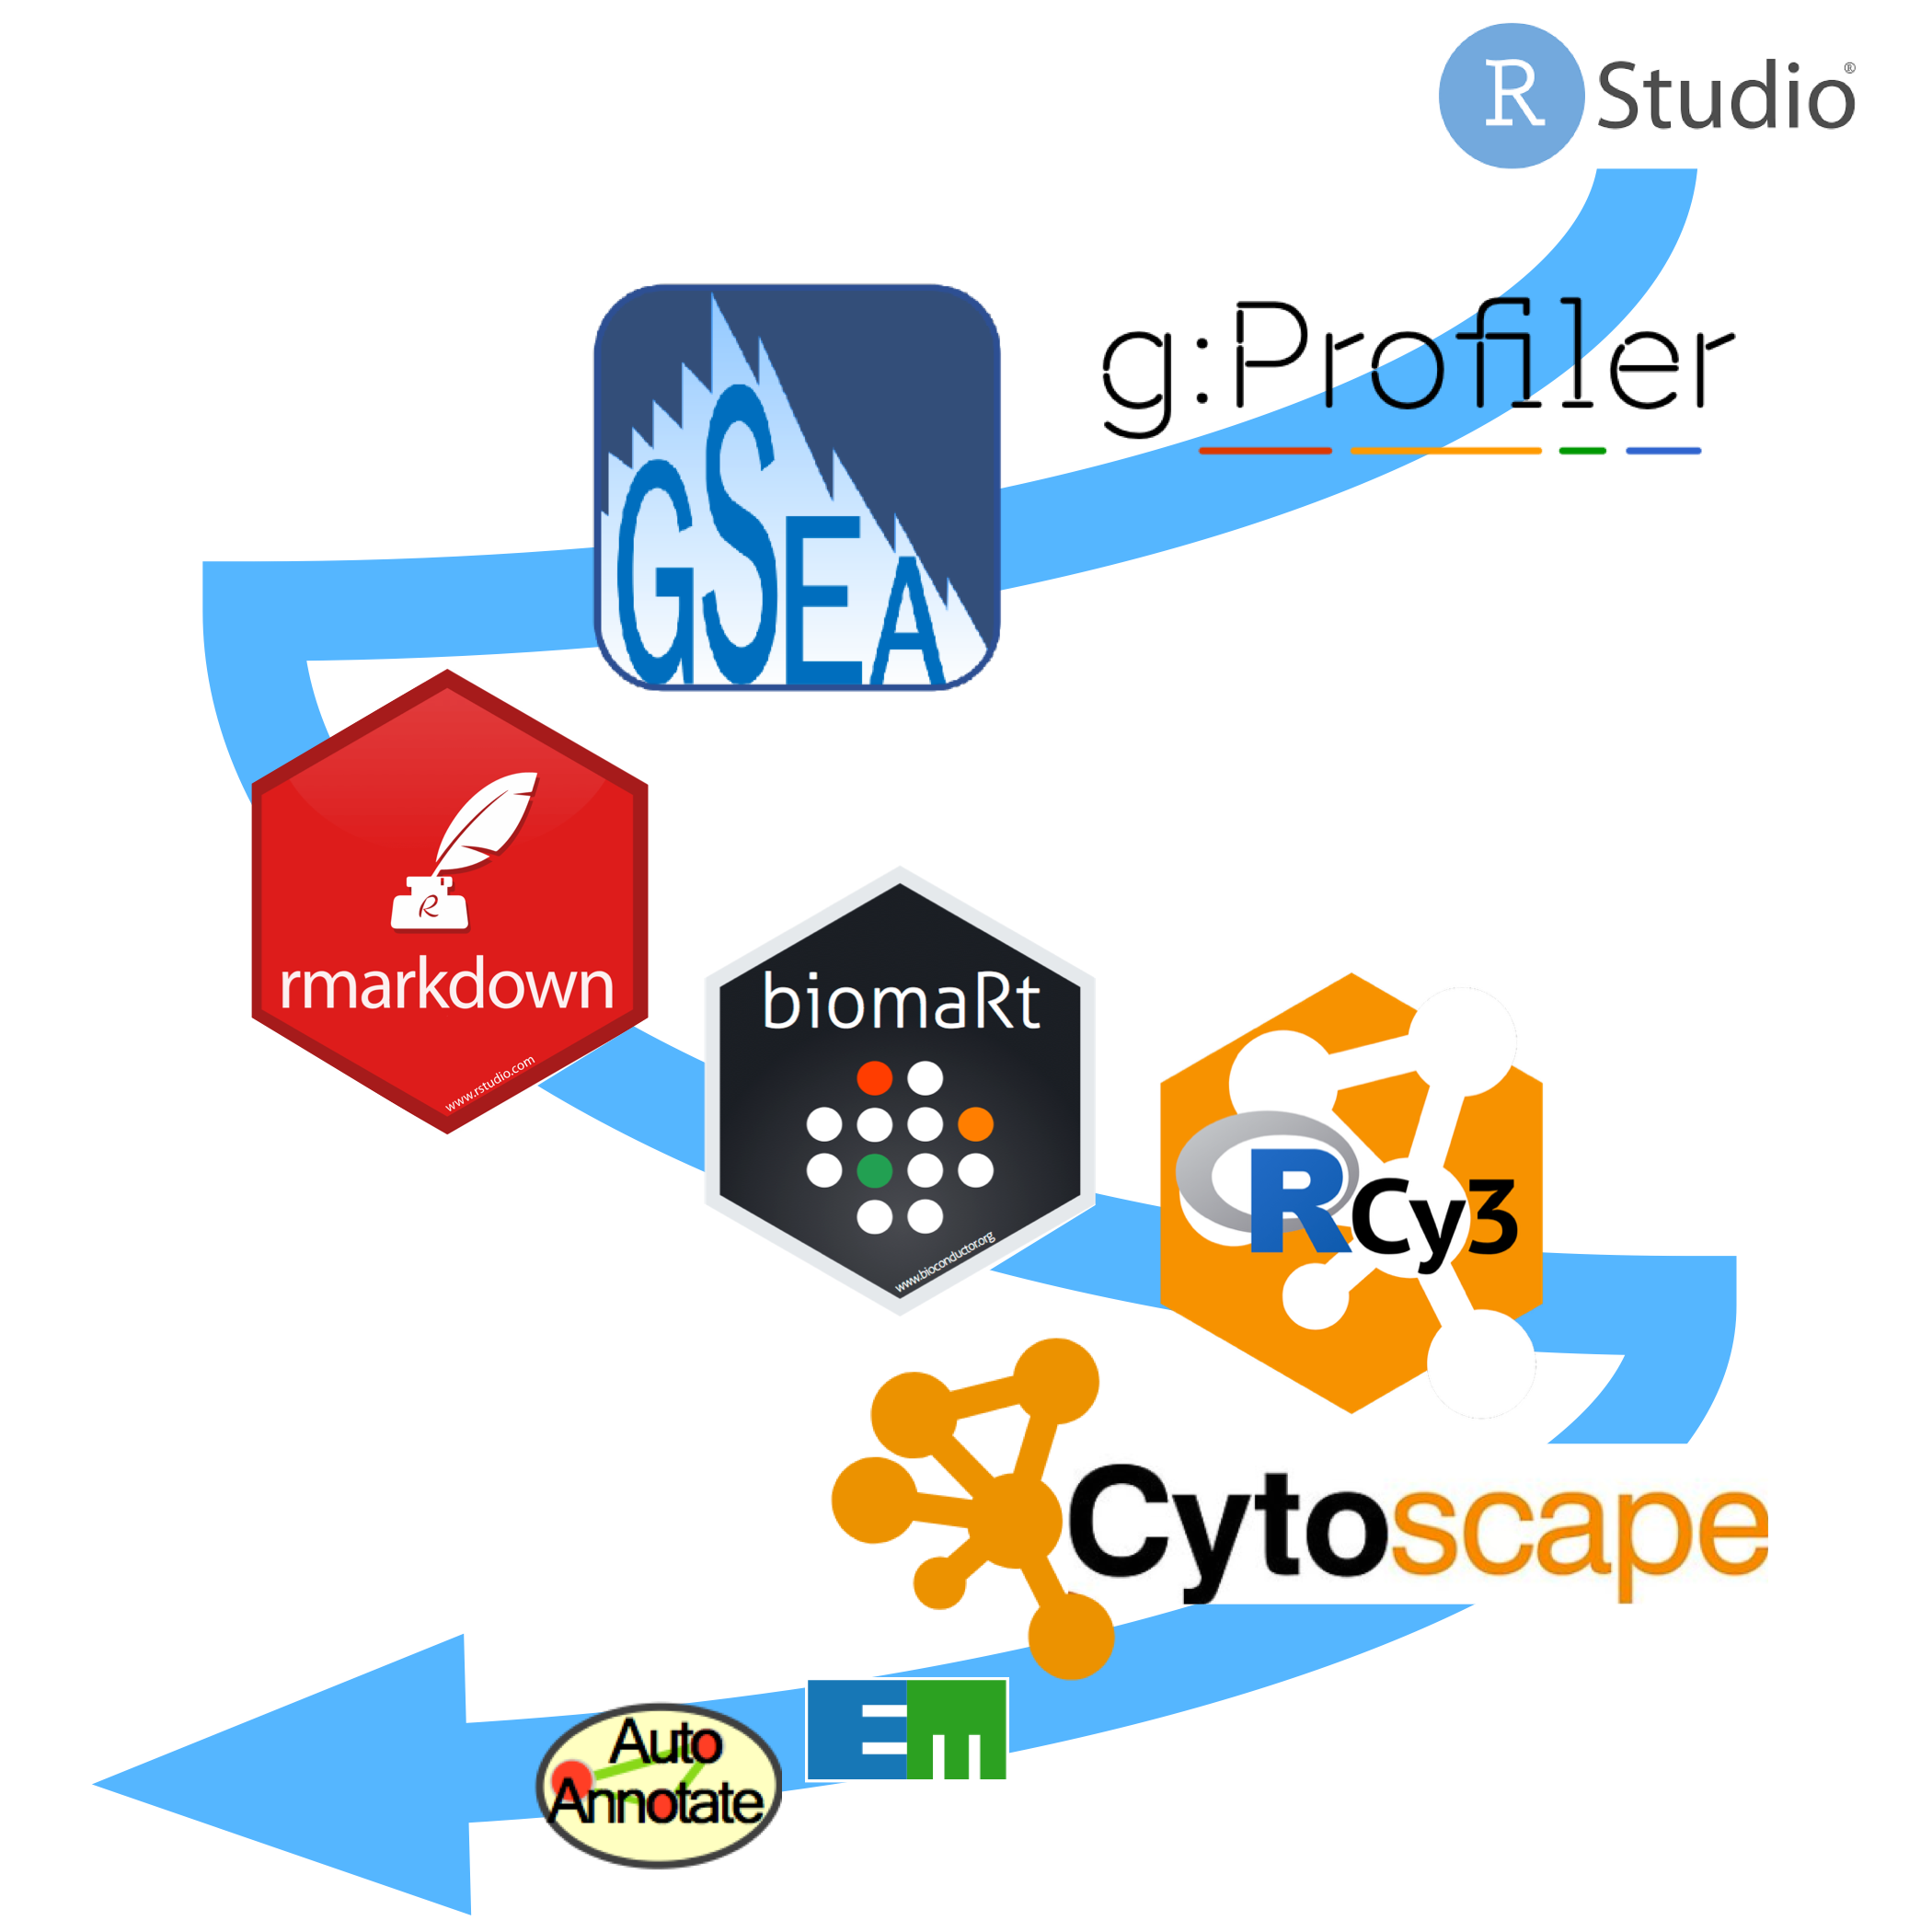
\includegraphics{./images/cover.png}

\chapter{Comparing GSEA and fGSEA}\label{intro}

Do you want to run the pathways and network analysis from R instead of doing everything mannually?

GSEA is a java application that can be run through their GUI or through the command line but is dependant on a java installation. There is no recent implementation of GSEA in R although there are many packages that perform similiar analysis.

Compare enrichment results from the GSEA java application and fast running R package fGSEA.

We are using the \textbf{bookdown} package (\citeproc{ref-R-bookdown}{Xie 2024}) in this Workshop R Notebooks book, which was built on top of R Markdown and \textbf{knitr} (\citeproc{ref-xie2015}{Xie 2015}).

\chapter{Setup}\label{setup}

\section{Install R and RStudio}\label{install-r-and-rstudio}

As with many open source projects, \textbf{R} is a constantly evolving language with regular updates. There is a major release once a year with patch releases through out the year. Often scripts and packages will work from one release to the next (ignoring pesky warnings that a package was compiled on a previous version of R is common) but there are exceptions. Some newer packages will only work on the latest version of \textbf{R} so sometimes the choice of upgrading or not using a new package might present themselves. Often, the amount of packages and work that is need to upgrade is not realized until the process has begun. This is where docker demonstrates it most valuable features. You can create a new instance based on the latest release of \textbf{R} and all your needed packages without having to change any of your current settings.

In order to use these notebooks supplied here you need to have:

\begin{itemize}
\tightlist
\item
  \textbf{R} installed on your computer and
\item
  a list of packages. (including BiocManager, BiomaRt, gprofiler2, GSA)
\end{itemize}

Each notebook in this set will check for the required packages and install them if they are missing so at the base level you need to just have \textbf{R} installed.

There are many different ways you can use and setup \textbf{R}.

\begin{enumerate}
\def\labelenumi{\arabic{enumi}.}
\tightlist
\item
  By simply installing \textbf{R} you can use it directly but
\item
  it is highly recommended that you also install and use \href{https://rstudio.com/products/rstudio/download/}{RStudio} which is an Integrate development environment (IDE) for \textbf{R}. You cannot just download RStudio and use it. It requires an installation of \textbf{R}.
\end{enumerate}

You don't need to install R and RStudio though. You can also use \textbf{R} and RStudio through docker. \textbf{I highly recommend using docker instead}

\section{Docker {[}Optional{]}}\label{docker-optional}

Changing versions and environments are a continuing struggle with bioinformatics pipelines and computational pipelines in general. An analysis written and performed a year ago might not run or produce the same results when it is run today. Recording package and system versions or not updating certain packages rarely work in the long run.

One the best solutions to reproducibility issues is containing your workflow or pipeline in its own coding environment where everything from the operating system, programs and packages are defined and can be built from a set of given instructions. There are many systems that offer this type of control including:

\begin{itemize}
\tightlist
\item
  \href{https://www.docker.com/}{Docker}.
\item
  \href{https://sylabs.io/}{Singularity}
\end{itemize}

``A container is a standard unit of software that packages up code and all its dependencies so the application runs quickly and reliably from one computing environment to another.'' (\citeproc{ref-docker}{{``What Is a Container?''} n.d.})

\textbf{Why are containers great for Bioiformatics?}

\begin{itemize}
\tightlist
\item
  allows you to create environments to run bioinformatis pipelines.
\item
  create a consistent environment to use for your pipelines.
\item
  test modifications to the pipeline without disrupting your current set up.
\item
  Coming back to an analysis years later and there is no need to install older versions of packages or programming languages. Simply create a container and re-run.
\end{itemize}

\section{Install Docker}\label{install-docker}

\begin{enumerate}
\def\labelenumi{\arabic{enumi}.}
\tightlist
\item
  Download and install \href{https://www.docker.com/products/docker-desktop}{docker desktop}.
\item
  Follow slightly different instructions for Windows or MacOS/Linux
\end{enumerate}

\subsection{Windows}\label{windows}

\begin{itemize}
\tightlist
\item
  it might prompt you to install additional updates (for example - \url{https://docs.Microsoft.com/en-us/windows/wsl/install-win10\#step-4---download-the-linux-kernel-update-package}) and require multiple restarts of your system or docker.
\item
  launch docker desktop app.
\item
  Open windows Power shell
\item
  navigate to directory on your system where you plan on keeping all your code. For example: C:\textbackslash USERS\textbackslash risserlin\textbackslash cbw\_workshop\_code
\item
  Run the following command: (the only difference with the windows command is the way the current directory is written. \$\{PWD\} instead of "\$(pwd)")
\end{itemize}

\begin{Shaded}
\begin{Highlighting}[]
\NormalTok{docker run }\SpecialCharTok{{-}}\NormalTok{e PASSWORD}\OtherTok{=}\NormalTok{changeit }\SpecialCharTok{{-}{-}}\NormalTok{rm \textbackslash{}}
  \SpecialCharTok{{-}}\NormalTok{v }\SpecialCharTok{$}\NormalTok{\{PWD\}}\SpecialCharTok{:}\ErrorTok{/}\NormalTok{home}\SpecialCharTok{/}\NormalTok{rstudio}\SpecialCharTok{/}\NormalTok{projects }\SpecialCharTok{{-}}\NormalTok{p }\DecValTok{8787}\SpecialCharTok{:}\DecValTok{8787}\NormalTok{ \textbackslash{}}
\NormalTok{  risserlin}\SpecialCharTok{/}\NormalTok{workshop\_base\_image}
\end{Highlighting}
\end{Shaded}

\begin{itemize}
\tightlist
\item
  Windows defender firewall might pop up with warning. Click on \emph{Allow access}.
\item
  In docker desktop you see all containers you are running and easily manage them.
\end{itemize}

\subsection{MacOS / Linux}\label{macos-linux}

\begin{itemize}
\tightlist
\item
  Open Terminal
\item
  navigate to directory on your system where you plan on keeping all your code. For example: /Users/risserlin/bcb420\_code
\item
  Run the following command: (the only difference with the windows command is the way the current directory is written. \$\{PWD\} instead of "\$(pwd)")
\end{itemize}

\begin{Shaded}
\begin{Highlighting}[]
\NormalTok{docker run }\SpecialCharTok{{-}}\NormalTok{e PASSWORD}\OtherTok{=}\NormalTok{changeit }\SpecialCharTok{{-}{-}}\NormalTok{rm \textbackslash{}}
  \SpecialCharTok{{-}}\NormalTok{v }\StringTok{"$(pwd)"}\SpecialCharTok{:}\ErrorTok{/}\NormalTok{home}\SpecialCharTok{/}\NormalTok{rstudio}\SpecialCharTok{/}\NormalTok{projects }\SpecialCharTok{{-}}\NormalTok{p }\DecValTok{8787}\SpecialCharTok{:}\DecValTok{8787}\NormalTok{ \textbackslash{}}
  \SpecialCharTok{{-}{-}}\NormalTok{add}\SpecialCharTok{{-}}\NormalTok{host }\StringTok{"localhost:My.IP.address"}
\NormalTok{  risserlin}\SpecialCharTok{/}\NormalTok{workshop\_base\_image}
\end{Highlighting}
\end{Shaded}

\chapter{Run GSEA from within R}\label{run-gsea-from-within-r}

This notebook is based largely on the \href{https://baderlab.github.io/Cytoscape_workflows/EnrichmentMapPipeline/Protocol2_createEM.html}{original notebook} published with EnrichmentMap Protocol(\citeproc{ref-em2019}{Reimand et al. 2019})

There is no package to run the original algorithm of GSEA(\citeproc{ref-gsea2005}{Subramanian et al. 2005}) in R. There are many packages that have been published to imitate the process but none are recognized by The GSEA team.\\
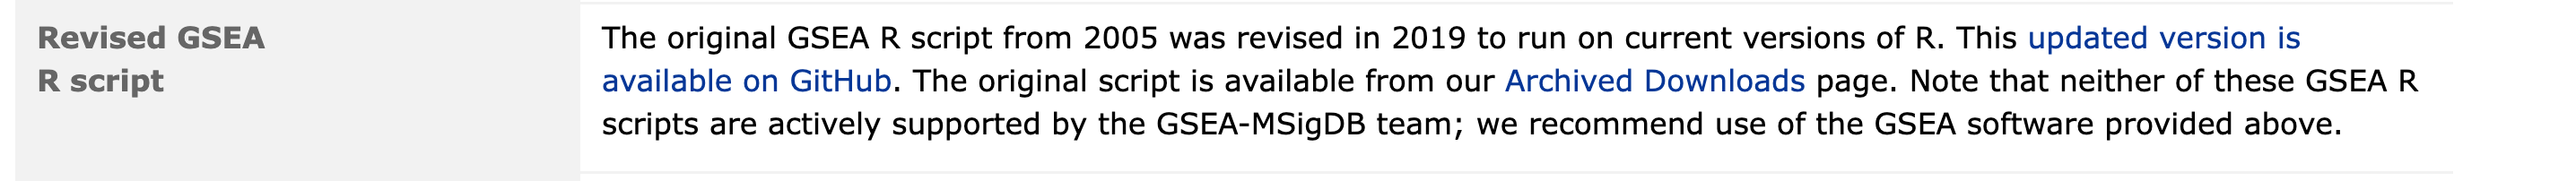
\includegraphics{./images/gsea_r_package_message.png}

\section{Load in required libraries}\label{load-in-required-libraries}

\begin{Shaded}
\begin{Highlighting}[]
\CommentTok{\#install required R and bioconductor packages}
\FunctionTok{tryCatch}\NormalTok{(}\AttributeTok{expr =}\NormalTok{ \{ }\FunctionTok{library}\NormalTok{(}\StringTok{"RCurl"}\NormalTok{)\}, }
         \AttributeTok{error =} \ControlFlowTok{function}\NormalTok{(e) \{  }
           \FunctionTok{install.packages}\NormalTok{(}\StringTok{"RCurl"}\NormalTok{)\}, }
         \AttributeTok{finally =} \FunctionTok{library}\NormalTok{(}\StringTok{"RCurl"}\NormalTok{))}
\end{Highlighting}
\end{Shaded}

\section{Configurable Parameters}\label{configurable-parameters}

In order to run GSEA automatically through the notebook you will need to download the gsea jar from \href{http://software.broadinstitute.org/gsea/downloads.jsp}{here}. Specify the exact path to the gsea jar in the parameters in order to automatically compute enrichments using GSEA.

If you are running this notebook using the \href{https://hub.docker.com/r/risserlin/workshop_base_image}{baderlab workshop docker image} then the image comes pre-installed with the gsea jar that you can use to run gsea directly in the docker. The path to the GSEA jar in the docker is - /home/rstudio/GSEA\_4.3.2/gsea-cli.sh

In order to run GSEA automatically you need to speciry the path to the gsea jar file.
The gsea\_jar needs to be the full path to the GSEA 4.3.3 directory that you downloaded from GSEA. for example /Users/johnsmith/GSEA\_4.3.3/gsea-cli.sh

The parameters are set manually here but if you want to run the script from the command line then you can update the notebook to pull the parameters from the command line given arguments by updating each variable below to pull the values from the paramters - for example:

\begin{itemize}
\tightlist
\item
  variable \textless- params\$parameter\_name
\end{itemize}

For more details see - \href{https://bookdown.org/yihui/rmarkdown/params-declare.html}{defining and using parameters} and \href{https://bookdown.org/yihui/rmarkdown/params-knit.html}{Knitting with parameters}

\begin{Shaded}
\begin{Highlighting}[]
\CommentTok{\#path to GSEA jar }
\CommentTok{\# defined in the paramters at top of notebook}
\NormalTok{gsea\_jar }\OtherTok{\textless{}{-}}\NormalTok{ params}\SpecialCharTok{$}\NormalTok{gsea\_jar}
\end{Highlighting}
\end{Shaded}

Set the working directory as the directory to the directory where you downloaded all protocol files. For example /User/JohnSmith/EMProtocolFiles/data

\begin{Shaded}
\begin{Highlighting}[]
\CommentTok{\# defined in the paramters at top of notebook}

\CommentTok{\#directory where all the data files are found.  For example {-}   ./data/ }
\NormalTok{working\_dir }\OtherTok{\textless{}{-}}\NormalTok{ params}\SpecialCharTok{$}\NormalTok{working\_dir}

\CommentTok{\#directory where all the data files are found.  For example {-}   ./generated\_data/gsea/}
\NormalTok{output\_dir }\OtherTok{\textless{}{-}}\NormalTok{ params}\SpecialCharTok{$}\NormalTok{output\_dir}
\ControlFlowTok{if}\NormalTok{(}\SpecialCharTok{!}\FunctionTok{dir.exists}\NormalTok{(output\_dir))\{}
  \FunctionTok{dir.create}\NormalTok{(output\_dir)}
\NormalTok{\}}

\CommentTok{\#The name to give the analysis in GSEA {-} for example Basal\_vs\_Classical}
\NormalTok{analysis\_name }\OtherTok{\textless{}{-}}\NormalTok{ params}\SpecialCharTok{$}\NormalTok{analysis\_name}

\CommentTok{\#rank file to use in GSEA analysis.  }
\CommentTok{\#For example {-} TCGA{-}PAAD\_GDC\_Subtype\_Moffitt\_BasalvsClassical\_ranks.rnk}
\NormalTok{rnk\_file }\OtherTok{\textless{}{-}}\NormalTok{ params}\SpecialCharTok{$}\NormalTok{rnk\_file}

\CommentTok{\#run\_gsea {-} true/false}
\CommentTok{\# This parameter is for the compilation of the notebook.  }
\NormalTok{run\_gsea }\OtherTok{\textless{}{-}}\NormalTok{ params}\SpecialCharTok{$}\NormalTok{run\_gsea}

\CommentTok{\#set the gmt file you want to use if you don\textquotesingle{}t want to use the latest gmt file.}
\CommentTok{\# For example, if you set dest\_gmt\_file =="" the below script will automatically}
\CommentTok{\# download the latest gmt file from baderlab webstie.  If it is set then it}
\CommentTok{\# will use the file specified.  }
\NormalTok{dest\_gmt\_file }\OtherTok{=} \StringTok{""}
\end{Highlighting}
\end{Shaded}

\section{Download the latest pathway definition file}\label{download-the-latest-pathway-definition-file}

Only Human, Mouse, Rat, and Woodchuck gene set files are currently available on the baderlab downloads site. If you are working with a species other than human (and it is either rat,mouse or woodchuck) change the gmt\_url below to the correct species. Check \href{http://download.baderlab.org/EM_Genesets/current_release/}{here} to see all available species.

To create your own GMT file using Ensembl see {[}Create GMT file from Ensembl{]}

\begin{Shaded}
\begin{Highlighting}[]
\ControlFlowTok{if}\NormalTok{(dest\_gmt\_file }\SpecialCharTok{==} \StringTok{""}\NormalTok{)\{}
\NormalTok{  gmt\_url }\OtherTok{=} \StringTok{"http://download.baderlab.org/EM\_Genesets/current\_release/Human/symbol/"}
  
  \CommentTok{\#list all the files on the server}
\NormalTok{  filenames }\OtherTok{=} \FunctionTok{getURL}\NormalTok{(gmt\_url)}
\NormalTok{  tc }\OtherTok{=} \FunctionTok{textConnection}\NormalTok{(filenames)}
\NormalTok{  contents }\OtherTok{=} \FunctionTok{readLines}\NormalTok{(tc)}
  \FunctionTok{close}\NormalTok{(tc)}
  
  \CommentTok{\#get the gmt that has all the pathways and does not include terms }
  \CommentTok{\# inferred from electronic annotations(IEA)}
  \CommentTok{\#start with gmt file that has pathways only and GO Biological Process only.}
\NormalTok{  rx }\OtherTok{=} \FunctionTok{gregexpr}\NormalTok{(}\StringTok{"(?\textless{}=\textless{}a href=}\SpecialCharTok{\textbackslash{}"}\StringTok{)(.*.GOBP\_AllPathways\_noPFOCR\_no\_GO\_iea.*.)(.gmt)(?=}\SpecialCharTok{\textbackslash{}"}\StringTok{\textgreater{})"}\NormalTok{,}
\NormalTok{    contents, }\AttributeTok{perl =} \ConstantTok{TRUE}\NormalTok{)}
\NormalTok{  gmt\_file }\OtherTok{=} \FunctionTok{unlist}\NormalTok{(}\FunctionTok{regmatches}\NormalTok{(contents, rx))}
  
\NormalTok{  dest\_gmt\_file }\OtherTok{\textless{}{-}} \FunctionTok{file.path}\NormalTok{(output\_dir,gmt\_file )}
  
  \CommentTok{\#check if this gmt file already exists}
  \ControlFlowTok{if}\NormalTok{(}\SpecialCharTok{!}\FunctionTok{file.exists}\NormalTok{(dest\_gmt\_file))\{}
    \FunctionTok{download.file}\NormalTok{(}
      \FunctionTok{paste}\NormalTok{(gmt\_url,gmt\_file,}\AttributeTok{sep=}\StringTok{""}\NormalTok{),}
      \AttributeTok{destfile=}\NormalTok{dest\_gmt\_file}
\NormalTok{    )}
\NormalTok{  \}}
\NormalTok{\}}
\end{Highlighting}
\end{Shaded}

\begin{center}\rule{0.5\linewidth}{0.5pt}\end{center}

\section{Run GSEA}\label{run-gsea}

(GSEA){[}\url{http://software.broadinstitute.org/gsea/index.jsp}{]} is a stand alone java program with many customizable options. It can be easily run through its integrated user interface. To make this a seemless pipeline we can run GSEA from the command line with a set of options. Any of the supplied options can be customized and there are many additional options that can be specified. For more details see (here){[}\url{http://software.broadinstitute.org/gsea/doc/GSEAUserGuideTEXT.htm\#_Running_GSEA_from}{]}

In the below command the following options have been specified:

\begin{itemize}
\tightlist
\item
  rnk - path to the rank file
\item
  gmx - path to the gene set definition (gmt) file
\item
  collapse - true/false indicates whether the expression/rnk file needs to be collapsed from probes to gene symbols
\item
  nperm - number of permutations
\item
  scoring\_scheme -
\item
  rpt\_label - name of the directory with output
\item
  rnd\_seed - random seed to use
\item
  set\_max - maximum size for individual gene sets. In GSEA interface this is set to 500 but we prefer to use a more stringent setting of 200.
\item
  set\_min - minimum size for individual gene sets
\item
  zip\_report - true/false to zip output directory
\item
  out - directory where to place the result directory.
\end{itemize}

\begin{Shaded}
\begin{Highlighting}[]
\NormalTok{start\_time }\OtherTok{\textless{}{-}} \FunctionTok{Sys.time}\NormalTok{()}

\ControlFlowTok{if}\NormalTok{(run\_gsea)\{}
\NormalTok{  command }\OtherTok{\textless{}{-}} \FunctionTok{paste}\NormalTok{(}\StringTok{""}\NormalTok{,gsea\_jar,  }
                   \StringTok{"GSEAPreRanked {-}gmx"}\NormalTok{, dest\_gmt\_file, }
                   \StringTok{"{-}rnk"}\NormalTok{ ,}\FunctionTok{file.path}\NormalTok{(working\_dir,rnk\_file), }
                   \StringTok{"{-}collapse false {-}nperm 1000 {-}scoring\_scheme weighted"}\NormalTok{, }
                   \StringTok{"{-}rpt\_label "}\NormalTok{,analysis\_name,}
                   \StringTok{"  {-}plot\_top\_x 20 {-}rnd\_seed 12345  {-}set\_max 500"}\NormalTok{,  }
                   \StringTok{" {-}set\_min 15 {-}zip\_report false "}\NormalTok{,}
                   \StringTok{" {-}out"}\NormalTok{ ,output\_dir, }
                   \StringTok{" \textgreater{} gsea\_output.txt"}\NormalTok{,}\AttributeTok{sep=}\StringTok{" "}\NormalTok{)}
  \FunctionTok{system}\NormalTok{(command)}
\NormalTok{\}}

\NormalTok{end\_time }\OtherTok{\textless{}{-}} \FunctionTok{Sys.time}\NormalTok{()}
\end{Highlighting}
\end{Shaded}

GSEA started at 2025-04-21 18:20:56.793255
GSEA finished at 2025-04-21 18:31:43.923337

GSEA total running time 10.7855013648669

\section{Create an Enrichment map of the top pathways.}\label{create-an-enrichment-map-of-the-top-pathways.}

\chapter{Run fGSEA from within R}\label{run-fgsea-from-within-r}

This notebook is based largely on the \href{https://baderlab.github.io/Cytoscape_workflows/EnrichmentMapPipeline/Protocol2_createEM.html}{original notebook} published with EnrichmentMap Protocol(\citeproc{ref-em2019}{Reimand et al. 2019})

\section{Load in required libraries}\label{load-in-required-libraries-1}

\begin{Shaded}
\begin{Highlighting}[]
\CommentTok{\#install required R and bioconductor packages}
\FunctionTok{tryCatch}\NormalTok{(}\AttributeTok{expr =}\NormalTok{ \{ }\FunctionTok{library}\NormalTok{(}\StringTok{"RCurl"}\NormalTok{)\}, }
         \AttributeTok{error =} \ControlFlowTok{function}\NormalTok{(e) \{  }
           \FunctionTok{install.packages}\NormalTok{(}\StringTok{"RCurl"}\NormalTok{)\}, }
         \AttributeTok{finally =} \FunctionTok{library}\NormalTok{(}\StringTok{"RCurl"}\NormalTok{))}

\FunctionTok{tryCatch}\NormalTok{(}\AttributeTok{expr =}\NormalTok{ \{ }\FunctionTok{library}\NormalTok{(}\StringTok{"fgsea"}\NormalTok{)\}, }
         \AttributeTok{error =} \ControlFlowTok{function}\NormalTok{(e) \{  }
           \FunctionTok{install.packages}\NormalTok{(}\StringTok{"fgsea"}\NormalTok{)\}, }
         \AttributeTok{finally =} \FunctionTok{library}\NormalTok{(}\StringTok{"fgsea"}\NormalTok{))}

\FunctionTok{tryCatch}\NormalTok{(}\AttributeTok{expr =}\NormalTok{ \{ }\FunctionTok{library}\NormalTok{(}\StringTok{"GSA"}\NormalTok{)\}, }
         \AttributeTok{error =} \ControlFlowTok{function}\NormalTok{(e) \{  }
           \FunctionTok{install.packages}\NormalTok{(}\StringTok{"GSA"}\NormalTok{)\}, }
         \AttributeTok{finally =} \FunctionTok{library}\NormalTok{(}\StringTok{"GSA"}\NormalTok{))}
\end{Highlighting}
\end{Shaded}

\section{function to write out fGSEA results}\label{function-to-write-out-fgsea-results}

Create function to write out fgsea results files for each sample

\begin{Shaded}
\begin{Highlighting}[]
\NormalTok{write\_sample\_fgsea\_results}\OtherTok{\textless{}{-}} \ControlFlowTok{function}\NormalTok{(current\_fgsea\_results, current\_results\_dir, }
\NormalTok{                                       current\_sample)\{}
    
\NormalTok{  current\_sample }\OtherTok{\textless{}{-}}\NormalTok{ current\_sample}
  
\NormalTok{    current\_sample\_directory\_fullpath }\OtherTok{\textless{}{-}} \FunctionTok{file.path}\NormalTok{(current\_results\_dir, current\_sample)}
    \ControlFlowTok{if}\NormalTok{(}\SpecialCharTok{!}\FunctionTok{dir.exists}\NormalTok{(current\_sample\_directory\_fullpath))\{}
      \FunctionTok{dir.create}\NormalTok{(current\_sample\_directory\_fullpath)}
\NormalTok{    \}}
  
    \CommentTok{\#calculate the rank at max}
    \CommentTok{\#fgsea returns the leading edge.  Just need to extract the highest rank from }
    \CommentTok{\# set to get the rank at max}
\NormalTok{    calculated\_rank\_at\_max }\OtherTok{\textless{}{-}} \FunctionTok{apply}\NormalTok{(current\_fgsea\_results,}\DecValTok{1}\NormalTok{,}\AttributeTok{FUN=}\ControlFlowTok{function}\NormalTok{(x)\{ }\FunctionTok{max}\NormalTok{(}\FunctionTok{which}\NormalTok{(}\FunctionTok{names}\NormalTok{(current\_ranks) }\SpecialCharTok{\%in\%} \FunctionTok{unlist}\NormalTok{(x[}\DecValTok{8}\NormalTok{])))\})}
    
    
\NormalTok{    fakeenr\_current\_sample }\OtherTok{\textless{}{-}} \FunctionTok{cbind}\NormalTok{(current\_fgsea\_results}\SpecialCharTok{$}\NormalTok{pathway,}
\NormalTok{                                     current\_fgsea\_results}\SpecialCharTok{$}\NormalTok{pathway,}
                                     \StringTok{"Details"}\NormalTok{,}
\NormalTok{                                     current\_fgsea\_results}\SpecialCharTok{$}\NormalTok{size,}
\NormalTok{                                     current\_fgsea\_results}\SpecialCharTok{$}\NormalTok{ES,}
\NormalTok{                                     current\_fgsea\_results}\SpecialCharTok{$}\NormalTok{NES,}
\NormalTok{                                     current\_fgsea\_results}\SpecialCharTok{$}\NormalTok{pval,}
\NormalTok{                                     current\_fgsea\_results}\SpecialCharTok{$}\NormalTok{padj,}
                                     \DecValTok{0}\NormalTok{,}
\NormalTok{                                     calculated\_rank\_at\_max,}
                                     \FunctionTok{apply}\NormalTok{(current\_fgsea\_results,}\DecValTok{1}\NormalTok{,}
                                           \AttributeTok{FUN=}\ControlFlowTok{function}\NormalTok{(x)\{}\FunctionTok{paste}\NormalTok{(}\FunctionTok{unlist}\NormalTok{(x[}\DecValTok{8}\NormalTok{]),}\AttributeTok{collapse=}\StringTok{","}\NormalTok{)\})) }
    
    \FunctionTok{colnames}\NormalTok{(fakeenr\_current\_sample) }\OtherTok{\textless{}{-}} \FunctionTok{c}\NormalTok{(}\StringTok{"name"}\NormalTok{,}\StringTok{"description"}\NormalTok{,}\StringTok{"GS details"}\NormalTok{,}\StringTok{"SIZE"}\NormalTok{,}\StringTok{"ES"}\NormalTok{,}\StringTok{"NES"}\NormalTok{,}\StringTok{"pval"}\NormalTok{,}\StringTok{"padj"}\NormalTok{,}\StringTok{"FWER"}\NormalTok{,}\StringTok{"Rank at Max"}\NormalTok{,}\StringTok{"leading edge genes"}\NormalTok{)}
    
\NormalTok{    fakeenr\_filename }\OtherTok{\textless{}{-}} \FunctionTok{paste0}\NormalTok{(current\_sample, }\StringTok{"\_fgsea\_enr\_results.txt"}\NormalTok{,}\AttributeTok{sep=}\StringTok{""}\NormalTok{)}
\NormalTok{    fakeenr\_filename\_docker }\OtherTok{\textless{}{-}} \FunctionTok{file.path}\NormalTok{(current\_sample\_directory\_fullpath,fakeenr\_filename)}
    
    \FunctionTok{write.table}\NormalTok{(fakeenr\_current\_sample ,}
\NormalTok{                fakeenr\_filename\_docker,}
                \AttributeTok{col.name=}\ConstantTok{TRUE}\NormalTok{,}\AttributeTok{sep=}\StringTok{"}\SpecialCharTok{\textbackslash{}t}\StringTok{"}\NormalTok{,}\AttributeTok{row.names=}\ConstantTok{FALSE}\NormalTok{,}\AttributeTok{quote=}\ConstantTok{FALSE}\NormalTok{,}\AttributeTok{fileEncoding=}\StringTok{"latin1"}\NormalTok{)}
    
    \CommentTok{\# "upload" the files to the host machine and replace each path with the host machine path}
    
    \CommentTok{\#create a fake expression file}
\NormalTok{    fakeexp }\OtherTok{\textless{}{-}} \FunctionTok{data.frame}\NormalTok{(}\AttributeTok{name =} \FunctionTok{names}\NormalTok{(current\_ranks), }
                          \AttributeTok{description =} \FunctionTok{names}\NormalTok{(current\_ranks),current\_ranks)}
\NormalTok{    fakeexp\_filename }\OtherTok{\textless{}{-}} \FunctionTok{paste0}\NormalTok{(current\_sample,}\StringTok{"fakeexpression.txt"}\NormalTok{,}\AttributeTok{sep=}\StringTok{""}\NormalTok{)}
\NormalTok{    fakeexp\_name\_docker }\OtherTok{\textless{}{-}} \FunctionTok{file.path}\NormalTok{( current\_sample\_directory\_fullpath,fakeexp\_filename)}

    \FunctionTok{write.table}\NormalTok{(fakeexp,}
\NormalTok{                fakeexp\_name\_docker,}
                \AttributeTok{col.name=}\ConstantTok{TRUE}\NormalTok{,}\AttributeTok{sep=}\StringTok{"}\SpecialCharTok{\textbackslash{}t}\StringTok{"}\NormalTok{,}\AttributeTok{row.names=}\ConstantTok{FALSE}\NormalTok{,}\AttributeTok{quote=}\ConstantTok{FALSE}\NormalTok{,}\AttributeTok{fileEncoding=}\StringTok{""}\NormalTok{)}
    
    
    \CommentTok{\#create a rank expression file}
\NormalTok{    fakernk }\OtherTok{\textless{}{-}} \FunctionTok{data.frame}\NormalTok{(}\AttributeTok{name =} \FunctionTok{names}\NormalTok{(current\_ranks), }
\NormalTok{                          current\_ranks)}
\NormalTok{    fakernk\_filename }\OtherTok{\textless{}{-}} \FunctionTok{paste0}\NormalTok{(current\_sample,}\StringTok{"fakeranks.rnk"}\NormalTok{,}\AttributeTok{sep=}\StringTok{""}\NormalTok{)}
\NormalTok{    fakernk\_name\_docker }\OtherTok{\textless{}{-}} \FunctionTok{file.path}\NormalTok{( current\_sample\_directory\_fullpath,fakernk\_filename)}

    \FunctionTok{write.table}\NormalTok{(fakernk,}
\NormalTok{                fakernk\_name\_docker,}
                \AttributeTok{col.name=}\ConstantTok{TRUE}\NormalTok{,}\AttributeTok{sep=}\StringTok{"}\SpecialCharTok{\textbackslash{}t}\StringTok{"}\NormalTok{,}\AttributeTok{row.names=}\ConstantTok{FALSE}\NormalTok{,}\AttributeTok{quote=}\ConstantTok{FALSE}\NormalTok{,}\AttributeTok{fileEncoding=}\StringTok{""}\NormalTok{)}
    
      
\NormalTok{\}}
\end{Highlighting}
\end{Shaded}

\section{Configurable Parameters}\label{configurable-parameters-1}

Set the working directory as the directory to the directory where you downloaded all protocol files. For example /User/JohnSmith/EMProtocolFiles/data

\begin{Shaded}
\begin{Highlighting}[]
\CommentTok{\# defined in the paramters at top of notebook}

\CommentTok{\#directory where all the data files are found.  For example {-}   ./data/ }
\NormalTok{working\_dir }\OtherTok{\textless{}{-}}\NormalTok{ params}\SpecialCharTok{$}\NormalTok{working\_dir}

\CommentTok{\#directory where all the data files are found.  For example {-}   ./generated\_data/gsea/}
\NormalTok{output\_dir }\OtherTok{\textless{}{-}}\NormalTok{ params}\SpecialCharTok{$}\NormalTok{output\_dir}
\ControlFlowTok{if}\NormalTok{(}\SpecialCharTok{!}\FunctionTok{exists}\NormalTok{(output\_dir))\{}
  \FunctionTok{dir.create}\NormalTok{(output\_dir)}
\NormalTok{\}}
\end{Highlighting}
\end{Shaded}

\begin{verbatim}
## Warning in dir.create(output_dir): './generated_data/fgsea' already exists
\end{verbatim}

\begin{Shaded}
\begin{Highlighting}[]
\CommentTok{\#The name to give the analysis in GSEA {-} for example Basal\_vs\_Classical}
\NormalTok{analysis\_name }\OtherTok{\textless{}{-}}\NormalTok{ params}\SpecialCharTok{$}\NormalTok{analysis\_name}

\CommentTok{\#rank file to use in GSEA analysis.  }
\CommentTok{\#For example {-} TCGA{-}PAAD\_GDC\_Subtype\_Moffitt\_BasalvsClassical\_ranks.rnk}
\NormalTok{rnk\_file }\OtherTok{\textless{}{-}}\NormalTok{ params}\SpecialCharTok{$}\NormalTok{rnk\_file}

\CommentTok{\#run\_gsea {-} true/false}
\CommentTok{\# This parameter is for the compilation of the notebook.  }
\NormalTok{run\_fgsea }\OtherTok{\textless{}{-}}\NormalTok{ params}\SpecialCharTok{$}\NormalTok{run\_fgsea}

\CommentTok{\#set the gmt file you want to use if you don\textquotesingle{}t want to use the latest gmt file.}
\CommentTok{\# For example, if you set dest\_gmt\_file =="" the below script will automatically}
\CommentTok{\# download the latest gmt file from baderlab webstie.  If it is set then it}
\CommentTok{\# will use the file specified.  }
\NormalTok{dest\_gmt\_file }\OtherTok{=} \StringTok{""}
\end{Highlighting}
\end{Shaded}

\section{Download the latest pathway definition file}\label{download-the-latest-pathway-definition-file-1}

Only Human, Mouse, Rat, and Woodchuck gene set files are currently available on the baderlab downloads site. If you are working with a species other than human (and it is either rat,mouse or woodchuck) change the gmt\_url below to the correct species. Check \href{http://download.baderlab.org/EM_Genesets/current_release/}{here} to see all available species.

To create your own GMT file using Ensembl see {[}Create GMT file from Ensembl{]}

\begin{Shaded}
\begin{Highlighting}[]
\ControlFlowTok{if}\NormalTok{(dest\_gmt\_file }\SpecialCharTok{==} \StringTok{""}\NormalTok{)\{}
\NormalTok{  gmt\_url }\OtherTok{=} \StringTok{"http://download.baderlab.org/EM\_Genesets/current\_release/Human/symbol/"}
  
  \CommentTok{\#list all the files on the server}
\NormalTok{  filenames }\OtherTok{=} \FunctionTok{getURL}\NormalTok{(gmt\_url)}
\NormalTok{  tc }\OtherTok{=} \FunctionTok{textConnection}\NormalTok{(filenames)}
\NormalTok{  contents }\OtherTok{=} \FunctionTok{readLines}\NormalTok{(tc)}
  \FunctionTok{close}\NormalTok{(tc)}
  
  \CommentTok{\#get the gmt that has all the pathways and does not include terms }
  \CommentTok{\# inferred from electronic annotations(IEA)}
  \CommentTok{\#start with gmt file that has pathways only and GO Biological Process only.}
\NormalTok{  rx }\OtherTok{=} \FunctionTok{gregexpr}\NormalTok{(}\StringTok{"(?\textless{}=\textless{}a href=}\SpecialCharTok{\textbackslash{}"}\StringTok{)(.*.GOBP\_AllPathways\_noPFOCR\_no\_GO\_iea.*.)(.gmt)(?=}\SpecialCharTok{\textbackslash{}"}\StringTok{\textgreater{})"}\NormalTok{,}
\NormalTok{    contents, }\AttributeTok{perl =} \ConstantTok{TRUE}\NormalTok{)}
\NormalTok{  gmt\_file }\OtherTok{=} \FunctionTok{unlist}\NormalTok{(}\FunctionTok{regmatches}\NormalTok{(contents, rx))}
  
\NormalTok{  dest\_gmt\_file }\OtherTok{\textless{}{-}} \FunctionTok{file.path}\NormalTok{(output\_dir,gmt\_file )}
  
  \CommentTok{\#check if this gmt file already exists}
  \ControlFlowTok{if}\NormalTok{(}\SpecialCharTok{!}\FunctionTok{file.exists}\NormalTok{(dest\_gmt\_file))\{}
    \FunctionTok{download.file}\NormalTok{(}
      \FunctionTok{paste}\NormalTok{(gmt\_url,gmt\_file,}\AttributeTok{sep=}\StringTok{""}\NormalTok{),}
      \AttributeTok{destfile=}\NormalTok{dest\_gmt\_file}
\NormalTok{    )}
\NormalTok{  \}}
\NormalTok{\}}


\CommentTok{\#load in the genesets.}
\FunctionTok{capture.output}\NormalTok{(all\_gs }\OtherTok{\textless{}{-}} \FunctionTok{GSA.read.gmt}\NormalTok{(dest\_gmt\_file) ,}\AttributeTok{file=}\StringTok{"gsa\_load.out"}\NormalTok{)}
\FunctionTok{names}\NormalTok{(all\_gs}\SpecialCharTok{$}\NormalTok{genesets) }\OtherTok{\textless{}{-}}\NormalTok{ all\_gs}\SpecialCharTok{$}\NormalTok{geneset.names}
\end{Highlighting}
\end{Shaded}

\begin{center}\rule{0.5\linewidth}{0.5pt}\end{center}

\section{Run fGSEA}\label{run-fgsea}

(fGSEA){[}\url{https://bioconductor.org/packages/release/bioc/html/fgsea.html}{]} is an R package that runs a fast Gene Set Enrichment Analysis.

In the below command the following options have been specified:

\begin{itemize}
\tightlist
\item
  rnk - path to the rank file
\item
  gmx - path to the gene set definition (gmt) file
\item
  collapse - true/false indicates whether the expression/rnk file needs to be collapsed from probes to gene symbols
\item
  nperm - number of permutations
\item
  scoring\_scheme -
\item
  rpt\_label - name of the directory with output
\item
  rnd\_seed - random seed to use
\item
  set\_max - maximum size for individual gene sets. In GSEA interface this is set to 500 but we prefer to use a more stringent setting of 200.
\item
  set\_min - minimum size for individual gene sets
\item
  zip\_report - true/false to zip output directory
\item
  out - directory where to place the result directory.
\end{itemize}

\begin{Shaded}
\begin{Highlighting}[]
\NormalTok{start\_time }\OtherTok{\textless{}{-}} \FunctionTok{Sys.time}\NormalTok{()}

\ControlFlowTok{if}\NormalTok{(run\_fgsea)\{}
  \CommentTok{\#get the subset of genes that are protein coding. }
\NormalTok{    current\_ranks }\OtherTok{\textless{}{-}} \FunctionTok{read.table}\NormalTok{(}\FunctionTok{file.path}\NormalTok{(working\_dir,rnk\_file),}\AttributeTok{header=}\ConstantTok{TRUE}\NormalTok{,}\AttributeTok{sep =} \StringTok{"}\SpecialCharTok{\textbackslash{}t}\StringTok{"}\NormalTok{)}
\NormalTok{    fgsea\_ranks }\OtherTok{\textless{}{-}}\NormalTok{ current\_ranks[,}\DecValTok{2}\NormalTok{]}
    \FunctionTok{names}\NormalTok{(fgsea\_ranks) }\OtherTok{\textless{}{-}}\NormalTok{ current\_ranks[,}\DecValTok{1}\NormalTok{]}
 
\NormalTok{    current\_ranks }\OtherTok{\textless{}{-}}\NormalTok{ fgsea\_ranks}
 
    \CommentTok{\#remove duplicated genes}
\NormalTok{    duplicated\_gene\_names }\OtherTok{\textless{}{-}}   
      \FunctionTok{names}\NormalTok{(current\_ranks)[}\FunctionTok{which}\NormalTok{(}\FunctionTok{duplicated}\NormalTok{(}\FunctionTok{names}\NormalTok{(current\_ranks)))]}
\NormalTok{    current\_ranks }\OtherTok{\textless{}{-}}\NormalTok{ current\_ranks[}\FunctionTok{which}\NormalTok{(}\SpecialCharTok{!}\FunctionTok{names}\NormalTok{(current\_ranks) }\SpecialCharTok{\%in\%} 
\NormalTok{                                           duplicated\_gene\_names)]}

\NormalTok{    current\_ranks }\OtherTok{\textless{}{-}} \FunctionTok{sort}\NormalTok{(current\_ranks,}\AttributeTok{decreasing =} \ConstantTok{TRUE}\NormalTok{)}
    \FunctionTok{set.seed}\NormalTok{(}\DecValTok{42}\NormalTok{)}
\NormalTok{    current\_fgsea\_results }\OtherTok{\textless{}{-}}\NormalTok{ fgsea}\SpecialCharTok{::}\FunctionTok{fgsea}\NormalTok{(all\_gs}\SpecialCharTok{$}\NormalTok{genesets, }
                                      \FunctionTok{sort}\NormalTok{(current\_ranks,}\AttributeTok{decreasing=}\ConstantTok{TRUE}\NormalTok{),}
                                      \AttributeTok{minSize=}\DecValTok{15}\NormalTok{,}
                                      \AttributeTok{maxSize =} \DecValTok{500}
\NormalTok{                                      )}
    
    \CommentTok{\#write out the fgsea results for this patient}
      \FunctionTok{write\_sample\_fgsea\_results}\NormalTok{(current\_fgsea\_results,output\_dir,analysis\_name)}
      

\NormalTok{\}}
\end{Highlighting}
\end{Shaded}

\begin{verbatim}
## Warning in write.table(fakeenr_current_sample, fakeenr_filename_docker, :
## invalid char string in output conversion
## Warning in write.table(fakeenr_current_sample, fakeenr_filename_docker, :
## invalid char string in output conversion
## Warning in write.table(fakeenr_current_sample, fakeenr_filename_docker, :
## invalid char string in output conversion
## Warning in write.table(fakeenr_current_sample, fakeenr_filename_docker, :
## invalid char string in output conversion
\end{verbatim}

\begin{Shaded}
\begin{Highlighting}[]
\NormalTok{end\_time }\OtherTok{\textless{}{-}} \FunctionTok{Sys.time}\NormalTok{()}
\end{Highlighting}
\end{Shaded}

GSEA started at 2025-04-21 18:32:04.383981
GSEA finished at 2025-04-21 18:32:21.759779

GSEA total running time 17.3757982254028

\begin{Shaded}
\begin{Highlighting}[]
\NormalTok{topPathwaysUp }\OtherTok{\textless{}{-}}\NormalTok{ current\_fgsea\_results[ES }\SpecialCharTok{\textgreater{}} \DecValTok{0}\NormalTok{][}\FunctionTok{head}\NormalTok{(}\FunctionTok{order}\NormalTok{(pval), }\AttributeTok{n=}\DecValTok{10}\NormalTok{), pathway]}
\NormalTok{topPathwaysDown }\OtherTok{\textless{}{-}}\NormalTok{ current\_fgsea\_results[ES }\SpecialCharTok{\textless{}} \DecValTok{0}\NormalTok{][}\FunctionTok{head}\NormalTok{(}\FunctionTok{order}\NormalTok{(pval), }\AttributeTok{n=}\DecValTok{10}\NormalTok{), pathway]}
\NormalTok{topPathways }\OtherTok{\textless{}{-}} \FunctionTok{c}\NormalTok{(topPathwaysUp, }\FunctionTok{rev}\NormalTok{(topPathwaysDown))}
\FunctionTok{plotGseaTable}\NormalTok{(all\_gs}\SpecialCharTok{$}\NormalTok{genesets[topPathways], current\_ranks, current\_fgsea\_results, }
              \AttributeTok{gseaParam=}\FloatTok{0.5}\NormalTok{)}
\end{Highlighting}
\end{Shaded}

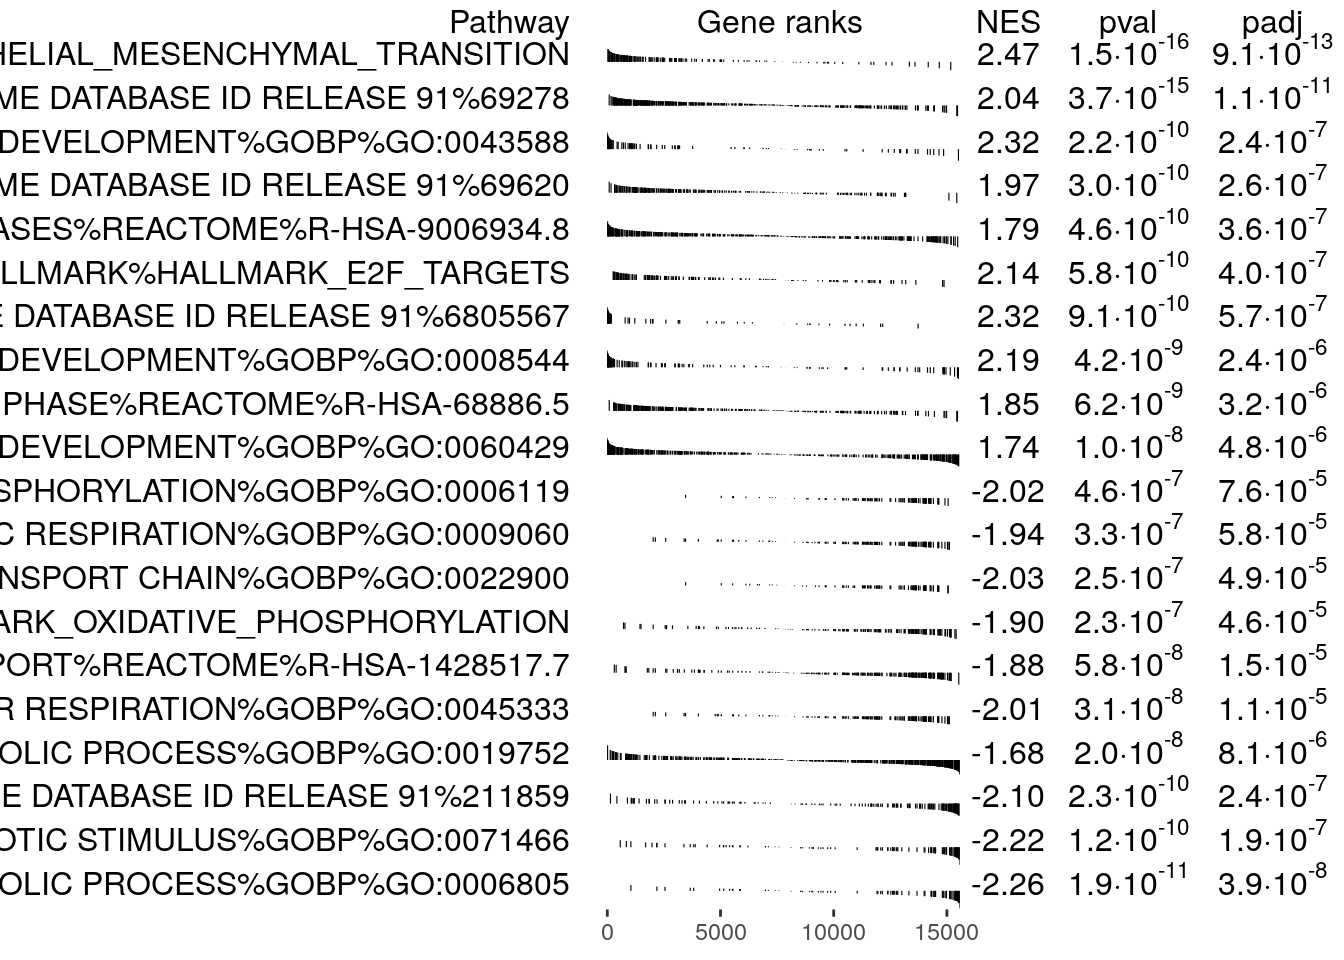
\includegraphics{04C-Timed_Run_fgsea_in_R_files/figure-latex/unnamed-chunk-2-1.pdf}

\section{Create an Enrichment map of the top pathways.}\label{create-an-enrichment-map-of-the-top-pathways.-1}

\chapter{Create Enrichment map from R with GSEA results}\label{create-enrichment-map-from-r-with-gsea-results}

\section{Initialize variables and libraries}\label{initialize-variables-and-libraries}

\begin{Shaded}
\begin{Highlighting}[]
\CommentTok{\#use library}
\CommentTok{\#make sure biocManager is installed}
\FunctionTok{tryCatch}\NormalTok{(}\AttributeTok{expr =}\NormalTok{ \{ }\FunctionTok{library}\NormalTok{(}\StringTok{"BiocManager"}\NormalTok{)\}, }
         \AttributeTok{error =} \ControlFlowTok{function}\NormalTok{(e) \{ }
           \FunctionTok{install.packages}\NormalTok{(}\StringTok{"BiocManager"}\NormalTok{)\}, }
         \AttributeTok{finally =} \FunctionTok{library}\NormalTok{(}\StringTok{"BiocManager"}\NormalTok{))}
\end{Highlighting}
\end{Shaded}

\begin{verbatim}
## Bioconductor version '3.19' is out-of-date; the current release version '3.21'
##   is available with R version '4.5'; see https://bioconductor.org/install
\end{verbatim}

\begin{Shaded}
\begin{Highlighting}[]
\FunctionTok{tryCatch}\NormalTok{(}\AttributeTok{expr =}\NormalTok{ \{ }\FunctionTok{library}\NormalTok{(}\StringTok{"ggplot2"}\NormalTok{)\}, }
         \AttributeTok{error =} \ControlFlowTok{function}\NormalTok{(e) \{ }\FunctionTok{install.packages}\NormalTok{(}\StringTok{"ggplot2"}\NormalTok{)\}, }
         \AttributeTok{finally =} \FunctionTok{library}\NormalTok{(}\StringTok{"ggplot2"}\NormalTok{))}

\CommentTok{\#use easy cyRest library to communicate with cytoscape.}
\FunctionTok{tryCatch}\NormalTok{(}\AttributeTok{expr =}\NormalTok{ \{ }\FunctionTok{library}\NormalTok{(}\StringTok{"RCy3"}\NormalTok{)\}, }
         \AttributeTok{error =} \ControlFlowTok{function}\NormalTok{(e) \{ BiocManager}\SpecialCharTok{::}\FunctionTok{install}\NormalTok{(}\StringTok{"RCy3"}\NormalTok{)\}, }
         \AttributeTok{finally =} \FunctionTok{library}\NormalTok{(}\StringTok{"RCy3"}\NormalTok{))}

\FunctionTok{tryCatch}\NormalTok{(}\AttributeTok{expr =}\NormalTok{ \{ }\FunctionTok{library}\NormalTok{(}\StringTok{"httr"}\NormalTok{)\}, }
         \AttributeTok{error =} \ControlFlowTok{function}\NormalTok{(e) \{ BiocManager}\SpecialCharTok{::}\FunctionTok{install}\NormalTok{(}\StringTok{"httr"}\NormalTok{)\}, }
         \AttributeTok{finally =} \FunctionTok{library}\NormalTok{(}\StringTok{"httr"}\NormalTok{))}
\end{Highlighting}
\end{Shaded}

\section{Configurable Parameters}\label{configurable-parameters-2}

\begin{Shaded}
\begin{Highlighting}[]
\CommentTok{\# is\_docker {-} true/false depending on if you are running R from docker}
\NormalTok{is\_docker }\OtherTok{\textless{}{-}} \ConstantTok{TRUE}

\CommentTok{\#directory where all the original input data file are}
\CommentTok{\# for example ./data/}
\NormalTok{working\_dir }\OtherTok{\textless{}{-}}\NormalTok{ params}\SpecialCharTok{$}\NormalTok{working\_dir}


\CommentTok{\#directory where all the generated data files are found.}
\CommentTok{\# For example {-} ./generated\_data/}
\CommentTok{\# If you are using all the notebooks from this set the generated data will be}
\CommentTok{\# put in the ./generated\_data folder.  You have to specify if it is gsea or }
\CommentTok{\# gprofiler}
\NormalTok{output\_dir }\OtherTok{\textless{}{-}}\NormalTok{ params}\SpecialCharTok{$}\NormalTok{output\_dir}


\CommentTok{\#defined threshold for GSEA enrichments }
\CommentTok{\#p{-}value to filter all the genesets.  For example {-}   1.0}
\NormalTok{pvalue\_gsea\_threshold }\OtherTok{\textless{}{-}}\NormalTok{ params}\SpecialCharTok{$}\NormalTok{pvalue\_thresh}

\CommentTok{\#q{-}value to filter all the genesets.  For example {-}   0.05}
\NormalTok{qvalue\_gsea\_threshold }\OtherTok{\textless{}{-}}\NormalTok{ params}\SpecialCharTok{$}\NormalTok{qvalue\_thresh}

\CommentTok{\#similarity threshold to filter all the genesets connections/edges.  }
\CommentTok{\# For example {-}   0.375}
\NormalTok{similarity\_threshold }\OtherTok{\textless{}{-}} \StringTok{"0.375"}

\CommentTok{\#similarity metric to filter all the genesets connections/edges }
\CommentTok{\# (can be OVERLAP, JACCARD, or COMBINED.   For example {-}   Combined}
\NormalTok{similarity\_metric }\OtherTok{=} \StringTok{"COMBINED"}
\end{Highlighting}
\end{Shaded}

\section{Specify Data files}\label{specify-data-files}

Depending on whether you are creating your enrichment map from g:Profiler or GSEA results the sets of files might be a little different. Minimally, you will need to specify:
* gmt file
* enrichment results file

Although there is a gmt file in the gsea edb results directory(which is the easiest method to create an enrichment map) it have been filtered to contain only genes represented in the expression set. If you use this fltered file you will get different pathway connectivity depending on the dataset being used. We recommend using original gmt file used for the gsea analysis and not the filtered one in the results directory.

\begin{Shaded}
\begin{Highlighting}[]
\CommentTok{\#use the newest gmt file in the output directory}
\NormalTok{gmt\_files }\OtherTok{\textless{}{-}} \FunctionTok{list.files}\NormalTok{(}\AttributeTok{path =}\NormalTok{ output\_dir, }\AttributeTok{pattern =} \StringTok{"}\SpecialCharTok{\textbackslash{}\textbackslash{}}\StringTok{.gmt"}\NormalTok{)}

  \CommentTok{\#get the details on the files}
\NormalTok{  details }\OtherTok{=} \FunctionTok{file.info}\NormalTok{(}\FunctionTok{file.path}\NormalTok{(output\_dir,gmt\_files))}
  \CommentTok{\#order according to newest to oldest}
\NormalTok{  details }\OtherTok{=}\NormalTok{ details[}\FunctionTok{with}\NormalTok{(details, }\FunctionTok{order}\NormalTok{(}\FunctionTok{as.POSIXct}\NormalTok{(mtime),}\AttributeTok{decreasing =} \ConstantTok{TRUE}\NormalTok{)), ]}

  \CommentTok{\#use the newest file:}
\NormalTok{ gmt\_gsea\_file }\OtherTok{\textless{}{-}} \FunctionTok{row.names}\NormalTok{(details)[}\DecValTok{1}\NormalTok{]}
\end{Highlighting}
\end{Shaded}

GSEA output directory - You can specify the exact name of the directory. The below code looks for the newest GSEA results directory and uses that.

\begin{Shaded}
\begin{Highlighting}[]
\NormalTok{gsea\_directories }\OtherTok{\textless{}{-}} \FunctionTok{list.files}\NormalTok{(}\AttributeTok{path =}\NormalTok{ output\_dir, }\AttributeTok{pattern =} \StringTok{"}\SpecialCharTok{\textbackslash{}\textbackslash{}}\StringTok{.GseaPreranked"}\NormalTok{)}

\CommentTok{\#get the details on the files}
\NormalTok{details }\OtherTok{=} \FunctionTok{file.info}\NormalTok{(}\FunctionTok{file.path}\NormalTok{(output\_dir,gsea\_directories))}
\CommentTok{\#order according to newest to oldest}
\NormalTok{details }\OtherTok{=}\NormalTok{ details[}\FunctionTok{with}\NormalTok{(details, }\FunctionTok{order}\NormalTok{(}\FunctionTok{as.POSIXct}\NormalTok{(mtime),}\AttributeTok{decreasing =} \ConstantTok{TRUE}\NormalTok{)), ]}

\CommentTok{\#use the newest file:}
\NormalTok{gsea\_output\_dir }\OtherTok{\textless{}{-}} \FunctionTok{row.names}\NormalTok{(details)[}\DecValTok{1}\NormalTok{]}

\NormalTok{gsea\_results\_path }\OtherTok{\textless{}{-}} \FunctionTok{file.path}\NormalTok{(gsea\_output\_dir,}\StringTok{"edb"}\NormalTok{)}
\NormalTok{gsea\_results\_filename }\OtherTok{\textless{}{-}} \FunctionTok{file.path}\NormalTok{(gsea\_results\_path,}\StringTok{"results.edb"}\NormalTok{)}
\end{Highlighting}
\end{Shaded}

\section{Optional File specification}\label{optional-file-specification}

These files are not needed to create the enrichment map but are very beneficial when analyzing your result.\\
* gene expression file
* gene ranks file

\begin{Shaded}
\begin{Highlighting}[]
\NormalTok{gsea\_ranks\_file }\OtherTok{\textless{}{-}} \FunctionTok{file.path}\NormalTok{(gsea\_results\_path,}
                             \FunctionTok{list.files}\NormalTok{(gsea\_results\_path,}\AttributeTok{pattern=}\StringTok{".rnk"}\NormalTok{))}

\NormalTok{expression\_file\_fullpath }\OtherTok{\textless{}{-}} \FunctionTok{file.path}\NormalTok{(working\_dir,}
\NormalTok{                          params}\SpecialCharTok{$}\NormalTok{expression\_file)}

\NormalTok{cls\_file\_fullpath }\OtherTok{\textless{}{-}} \FunctionTok{file.path}\NormalTok{(working\_dir, params}\SpecialCharTok{$}\NormalTok{cls\_file)}

\CommentTok{\#define an analysis name}
\NormalTok{cur\_model\_name }\OtherTok{\textless{}{-}}\NormalTok{ params}\SpecialCharTok{$}\NormalTok{analysis\_name}
\end{Highlighting}
\end{Shaded}

\section{Launch Cytoscape}\label{launch-cytoscape}

Launch Cytoscape (by default cytoscape will automatically enable rest so as long as cytoscape 3.3 or higher is open R should be able to communicate with it). Make sure if you get an message asking you if you want communicate with other apps that you select ``Allow''.

\section{Make sure you can connect to Cytoscape}\label{make-sure-you-can-connect-to-cytoscape}

\begin{Shaded}
\begin{Highlighting}[]
\ControlFlowTok{if}\NormalTok{(is\_docker)\{}
\NormalTok{  current\_base }\OtherTok{=} \StringTok{"host.docker.internal:1234/v1"}
\NormalTok{  .defaultBaseUrl }\OtherTok{\textless{}{-}} \StringTok{"http://host.docker.internal:1234/v1"}
\NormalTok{\} }\ControlFlowTok{else}\NormalTok{\{}
\NormalTok{  current\_base }\OtherTok{=} \StringTok{"localhost:1234/v1"}
\NormalTok{\}}

\FunctionTok{cytoscapePing}\NormalTok{ (}\AttributeTok{base.url =}\NormalTok{ current\_base)}
\end{Highlighting}
\end{Shaded}

\begin{verbatim}
## You are connected to Cytoscape!
\end{verbatim}

\begin{Shaded}
\begin{Highlighting}[]
\FunctionTok{cytoscapeVersionInfo}\NormalTok{ (}\AttributeTok{base.url =}\NormalTok{ current\_base)}
\end{Highlighting}
\end{Shaded}

\begin{verbatim}
##       apiVersion cytoscapeVersion 
##             "v1"         "3.10.3"
\end{verbatim}

\begin{center}\rule{0.5\linewidth}{0.5pt}\end{center}

\section{Create an Enrichment map}\label{create-an-enrichment-map}

If you are running R from within a docker you need to first upload your datafiles to Cytoscape before you can create your enrichment map

\begin{Shaded}
\begin{Highlighting}[]
\CommentTok{\#if using docker we need to replace all the the paths to the host path}
\ControlFlowTok{if}\NormalTok{(is\_docker) \{}
\NormalTok{  upload\_em\_file }\OtherTok{\textless{}{-}} \ControlFlowTok{function}\NormalTok{(localPath) \{}
\NormalTok{    bname }\OtherTok{\textless{}{-}} \FunctionTok{basename}\NormalTok{(localPath)}
\NormalTok{    r }\OtherTok{\textless{}{-}} \FunctionTok{POST}\NormalTok{(}
      \AttributeTok{url =} 
\FunctionTok{paste}\NormalTok{(}\StringTok{\textquotesingle{}http://host.docker.internal:1234/enrichmentmap/textfileupload?fileName=\textquotesingle{}}\NormalTok{, }
\NormalTok{                  bname, }\AttributeTok{sep=}\StringTok{""}\NormalTok{),}
      \AttributeTok{config =} \FunctionTok{list}\NormalTok{(),}
      \AttributeTok{body =} \FunctionTok{list}\NormalTok{(}\AttributeTok{file =} \FunctionTok{upload\_file}\NormalTok{(localPath)),}
      \AttributeTok{encode =} \StringTok{"multipart"}\NormalTok{,}
      \AttributeTok{handle =} \ConstantTok{NULL}
\NormalTok{    )}
    \FunctionTok{content}\NormalTok{(r,}\StringTok{"parsed"}\NormalTok{)}\SpecialCharTok{$}\NormalTok{path}
\NormalTok{  \}}
  
  \CommentTok{\# "upload" the files to the host machine and replace each path }
  \CommentTok{\# with the host machine path}
\NormalTok{  expression\_file\_fullpath }\OtherTok{\textless{}{-}} \FunctionTok{upload\_em\_file}\NormalTok{(expression\_file\_fullpath)}
\NormalTok{  class\_file\_fullpath }\OtherTok{\textless{}{-}} \FunctionTok{upload\_em\_file}\NormalTok{(cls\_file\_fullpath)}
\NormalTok{  gmt\_gsea\_file }\OtherTok{\textless{}{-}} \FunctionTok{upload\_em\_file}\NormalTok{(gmt\_gsea\_file)}
\NormalTok{  gsea\_ranks\_file }\OtherTok{\textless{}{-}} \FunctionTok{upload\_em\_file}\NormalTok{(gsea\_ranks\_file)}
\NormalTok{  gsea\_results\_filename }\OtherTok{\textless{}{-}} \FunctionTok{upload\_em\_file}\NormalTok{(gsea\_results\_filename)}
\NormalTok{\}}
\end{Highlighting}
\end{Shaded}

\begin{center}\rule{0.5\linewidth}{0.5pt}\end{center}

\section{Create an Enrichment map - run EM command}\label{create-an-enrichment-map---run-em-command}

\begin{Shaded}
\begin{Highlighting}[]
\DocumentationTok{\#\#\#\#\#\#\#\#\#\#\#\#\#\#\#\#\#\#\#\#\#\#\#\#\#\#\#\#\#\#\#\#\#\#\#\#\#\#\#}
\CommentTok{\#create EM}
\NormalTok{current\_network\_name }\OtherTok{\textless{}{-}} \FunctionTok{paste}\NormalTok{(cur\_model\_name,pvalue\_gsea\_threshold,}
\NormalTok{                              qvalue\_gsea\_threshold,}\AttributeTok{sep=}\StringTok{"\_"}\NormalTok{)}

\NormalTok{em\_command }\OtherTok{=} \FunctionTok{paste}\NormalTok{(}\StringTok{\textquotesingle{}enrichmentmap build analysisType="gsea" gmtFile=\textquotesingle{}}\NormalTok{,}
\NormalTok{                                                              gmt\_gsea\_file,}
                   \StringTok{\textquotesingle{}pvalue=\textquotesingle{}}\NormalTok{,pvalue\_gsea\_threshold, }
                   \StringTok{\textquotesingle{}qvalue=\textquotesingle{}}\NormalTok{,qvalue\_gsea\_threshold,}
                   \StringTok{\textquotesingle{}similaritycutoff=\textquotesingle{}}\NormalTok{,similarity\_threshold,}
                   \StringTok{\textquotesingle{}coefficients=\textquotesingle{}}\NormalTok{,similarity\_metric,}
                   \StringTok{\textquotesingle{}ranksDataset1=\textquotesingle{}}\NormalTok{, gsea\_ranks\_file,}
                   \StringTok{\textquotesingle{}enrichmentsDataset1=\textquotesingle{}}\NormalTok{,gsea\_results\_filename, }
                   \StringTok{\textquotesingle{}filterByExpressions=false\textquotesingle{}}\NormalTok{,}
                   \StringTok{\textquotesingle{}expressionDataset1=\textquotesingle{}}\NormalTok{,expression\_file\_fullpath,}
                   \StringTok{\textquotesingle{}classDataset1=\textquotesingle{}}\NormalTok{,class\_file\_fullpath,}
                   \StringTok{\textquotesingle{}gmtFile=\textquotesingle{}}\NormalTok{,gmt\_gsea\_file,}
                   \AttributeTok{sep=}\StringTok{" "}\NormalTok{)}

\CommentTok{\#enrichment map command will return the suid of newly created network.}
\NormalTok{response }\OtherTok{\textless{}{-}} \FunctionTok{commandsGET}\NormalTok{(em\_command,}\AttributeTok{base.url =}\NormalTok{ current\_base)}

\NormalTok{current\_network\_suid }\OtherTok{\textless{}{-}} \DecValTok{0}
\CommentTok{\#enrichment map command will return the suid of newly created network }
\CommentTok{\# unless it Failed.  If it failed it will contain the word failed}
\ControlFlowTok{if}\NormalTok{(}\FunctionTok{grepl}\NormalTok{(}\AttributeTok{pattern=}\StringTok{"Failed"}\NormalTok{, response))\{}
  \FunctionTok{paste}\NormalTok{(response)}
\NormalTok{\} }\ControlFlowTok{else}\NormalTok{ \{}
\NormalTok{  current\_network\_suid }\OtherTok{\textless{}{-}}\NormalTok{ response}
\NormalTok{\}}

\CommentTok{\#check to see if the network name is unique}
\NormalTok{current\_names }\OtherTok{\textless{}{-}} \FunctionTok{getNetworkList}\NormalTok{(}\AttributeTok{base.url =}\NormalTok{ current\_base)}
\ControlFlowTok{if}\NormalTok{(current\_network\_name }\SpecialCharTok{\%in\%}\NormalTok{ current\_names)\{}
  \CommentTok{\#if the name already exists in the network names then put the SUID in front}
  \CommentTok{\# of the name (this does not work if you put the suid at the end of the name)}
\NormalTok{  current\_network\_name }\OtherTok{\textless{}{-}} \FunctionTok{paste}\NormalTok{(current\_network\_suid,}
\NormalTok{                                current\_network\_name,}\AttributeTok{sep=}\StringTok{"\_"}\NormalTok{)}
\NormalTok{\}}
\NormalTok{response }\OtherTok{\textless{}{-}} \FunctionTok{renameNetwork}\NormalTok{(}\AttributeTok{title=}\NormalTok{current\_network\_name, }
                       \AttributeTok{network =} \FunctionTok{as.numeric}\NormalTok{(current\_network\_suid),}
                       \AttributeTok{base.url =}\NormalTok{ current\_base)}
\end{Highlighting}
\end{Shaded}

\section{Get a screen shot of the initial network.}\label{get-a-screen-shot-of-the-initial-network.}

\begin{Shaded}
\begin{Highlighting}[]
\CommentTok{\#you can only output the file if it isn\textquotesingle{}t on docker}
\CommentTok{\#on docker is put it into the user\textquotesingle{}s home directory with docker }
\CommentTok{\# has not access to}
\ControlFlowTok{if}\NormalTok{(}\SpecialCharTok{!}\NormalTok{is\_docker)\{}
\NormalTok{  output\_network\_file }\OtherTok{\textless{}{-}} \FunctionTok{file.path}\NormalTok{(}\FunctionTok{getwd}\NormalTok{(),}\StringTok{"initial\_screenshot\_network.png"}\NormalTok{)}
\NormalTok{  output\_network\_file\_current }\OtherTok{\textless{}{-}}\NormalTok{ output\_network\_file}

  \FunctionTok{fitContent}\NormalTok{()}

  \ControlFlowTok{if}\NormalTok{(}\FunctionTok{file.exists}\NormalTok{(output\_network\_file))\{}
    \CommentTok{\#cytoscape hangs waiting for user response if file already exists.}
    \CommentTok{\# Remove it first}
\NormalTok{    response }\OtherTok{\textless{}{-}} \FunctionTok{file.remove}\NormalTok{(output\_network\_file)}
\NormalTok{  \} }

\NormalTok{  response }\OtherTok{\textless{}{-}} \FunctionTok{exportImage}\NormalTok{(output\_network\_file, }\AttributeTok{type =} \StringTok{"png"}\NormalTok{,}
                          \AttributeTok{base.url =}\NormalTok{ current\_base)}
\NormalTok{\}}
\end{Highlighting}
\end{Shaded}

\chapter{Create Enrichment map from R with GSEA results}\label{create-enrichment-map-from-r-with-gsea-results-1}

\section{Initialize variables and libraries}\label{initialize-variables-and-libraries-1}

\begin{Shaded}
\begin{Highlighting}[]
\CommentTok{\#use library}
\CommentTok{\#make sure biocManager is installed}
\FunctionTok{tryCatch}\NormalTok{(}\AttributeTok{expr =}\NormalTok{ \{ }\FunctionTok{library}\NormalTok{(}\StringTok{"BiocManager"}\NormalTok{)\}, }
         \AttributeTok{error =} \ControlFlowTok{function}\NormalTok{(e) \{ }
           \FunctionTok{install.packages}\NormalTok{(}\StringTok{"BiocManager"}\NormalTok{)\}, }
         \AttributeTok{finally =} \FunctionTok{library}\NormalTok{(}\StringTok{"BiocManager"}\NormalTok{))}
\end{Highlighting}
\end{Shaded}

\begin{verbatim}
## Bioconductor version '3.19' is out-of-date; the current release version '3.21'
##   is available with R version '4.5'; see https://bioconductor.org/install
\end{verbatim}

\begin{Shaded}
\begin{Highlighting}[]
\FunctionTok{tryCatch}\NormalTok{(}\AttributeTok{expr =}\NormalTok{ \{ }\FunctionTok{library}\NormalTok{(}\StringTok{"ggplot2"}\NormalTok{)\}, }
         \AttributeTok{error =} \ControlFlowTok{function}\NormalTok{(e) \{ }\FunctionTok{install.packages}\NormalTok{(}\StringTok{"ggplot2"}\NormalTok{)\}, }
         \AttributeTok{finally =} \FunctionTok{library}\NormalTok{(}\StringTok{"ggplot2"}\NormalTok{))}

\CommentTok{\#use easy cyRest library to communicate with cytoscape.}
\FunctionTok{tryCatch}\NormalTok{(}\AttributeTok{expr =}\NormalTok{ \{ }\FunctionTok{library}\NormalTok{(}\StringTok{"RCy3"}\NormalTok{)\}, }
         \AttributeTok{error =} \ControlFlowTok{function}\NormalTok{(e) \{ BiocManager}\SpecialCharTok{::}\FunctionTok{install}\NormalTok{(}\StringTok{"RCy3"}\NormalTok{)\}, }
         \AttributeTok{finally =} \FunctionTok{library}\NormalTok{(}\StringTok{"RCy3"}\NormalTok{))}

\FunctionTok{tryCatch}\NormalTok{(}\AttributeTok{expr =}\NormalTok{ \{ }\FunctionTok{library}\NormalTok{(}\StringTok{"httr"}\NormalTok{)\}, }
         \AttributeTok{error =} \ControlFlowTok{function}\NormalTok{(e) \{ BiocManager}\SpecialCharTok{::}\FunctionTok{install}\NormalTok{(}\StringTok{"httr"}\NormalTok{)\}, }
         \AttributeTok{finally =} \FunctionTok{library}\NormalTok{(}\StringTok{"httr"}\NormalTok{))}
\end{Highlighting}
\end{Shaded}

\section{Configurable Parameters}\label{configurable-parameters-3}

\begin{Shaded}
\begin{Highlighting}[]
\CommentTok{\# is\_docker {-} true/false depending on if you are running R from docker}
\NormalTok{is\_docker }\OtherTok{\textless{}{-}} \ConstantTok{TRUE}

\CommentTok{\#directory where all the original input data file are}
\CommentTok{\# for example ./data/}
\NormalTok{working\_dir }\OtherTok{\textless{}{-}}\NormalTok{ params}\SpecialCharTok{$}\NormalTok{working\_dir}


\CommentTok{\#directory where all the generated data files are found.}
\CommentTok{\# For example {-} ./generated\_data/}
\CommentTok{\# If you are using all the notebooks from this set the generated data will be}
\CommentTok{\# put in the ./generated\_data folder.  You have to specify if it is gsea or }
\CommentTok{\# gprofiler}
\NormalTok{output\_dir }\OtherTok{\textless{}{-}}\NormalTok{ params}\SpecialCharTok{$}\NormalTok{output\_dir}


\CommentTok{\#defined threshold for GSEA enrichments }
\CommentTok{\#p{-}value to filter all the genesets.  For example {-}   1.0}
\NormalTok{pvalue\_gsea\_threshold }\OtherTok{\textless{}{-}}\NormalTok{ params}\SpecialCharTok{$}\NormalTok{pvalue\_thresh}

\CommentTok{\#q{-}value to filter all the genesets.  For example {-}   0.05}
\NormalTok{qvalue\_gsea\_threshold }\OtherTok{\textless{}{-}}\NormalTok{ params}\SpecialCharTok{$}\NormalTok{qvalue\_thresh}

\CommentTok{\#similarity threshold to filter all the genesets connections/edges.  }
\CommentTok{\# For example {-}   0.375}
\NormalTok{similarity\_threshold }\OtherTok{\textless{}{-}} \StringTok{"0.375"}

\CommentTok{\#similarity metric to filter all the genesets connections/edges }
\CommentTok{\# (can be OVERLAP, JACCARD, or COMBINED.   For example {-}   Combined}
\NormalTok{similarity\_metric }\OtherTok{=} \StringTok{"COMBINED"}
\end{Highlighting}
\end{Shaded}

\section{Specify Data files}\label{specify-data-files-1}

Depending on whether you are creating your enrichment map from g:Profiler or GSEA results the sets of files might be a little different. Minimally, you will need to specify:
* gmt file
* enrichment results file

Although there is a gmt file in the gsea edb results directory(which is the easiest method to create an enrichment map) it have been filtered to contain only genes represented in the expression set. If you use this fltered file you will get different pathway connectivity depending on the dataset being used. We recommend using original gmt file used for the gsea analysis and not the filtered one in the results directory.

\begin{Shaded}
\begin{Highlighting}[]
\CommentTok{\#use the newest gmt file in the output directory}
\NormalTok{gmt\_files }\OtherTok{\textless{}{-}} \FunctionTok{list.files}\NormalTok{(}\AttributeTok{path =}\NormalTok{ output\_dir, }\AttributeTok{pattern =} \StringTok{"}\SpecialCharTok{\textbackslash{}\textbackslash{}}\StringTok{.gmt"}\NormalTok{)}

  \CommentTok{\#get the details on the files}
\NormalTok{  details }\OtherTok{=} \FunctionTok{file.info}\NormalTok{(}\FunctionTok{file.path}\NormalTok{(output\_dir,gmt\_files))}
  \CommentTok{\#order according to newest to oldest}
\NormalTok{  details }\OtherTok{=}\NormalTok{ details[}\FunctionTok{with}\NormalTok{(details, }\FunctionTok{order}\NormalTok{(}\FunctionTok{as.POSIXct}\NormalTok{(mtime),}\AttributeTok{decreasing =} \ConstantTok{TRUE}\NormalTok{)), ]}

  \CommentTok{\#use the newest file:}
\NormalTok{ gmt\_gsea\_file }\OtherTok{\textless{}{-}} \FunctionTok{row.names}\NormalTok{(details)[}\DecValTok{1}\NormalTok{]}
\end{Highlighting}
\end{Shaded}

fGSEA output directory - You can specify the exact name of the directory. The below code looks for the newest GSEA results directory and uses that.

\begin{Shaded}
\begin{Highlighting}[]
\NormalTok{gsea\_directories }\OtherTok{\textless{}{-}} \FunctionTok{list.files}\NormalTok{(}\AttributeTok{path =}\NormalTok{ output\_dir)}

\CommentTok{\#get the details on the files}
\NormalTok{details }\OtherTok{=} \FunctionTok{file.info}\NormalTok{(}\FunctionTok{file.path}\NormalTok{(output\_dir,gsea\_directories))}
\CommentTok{\#order according to newest to oldest}
\NormalTok{details }\OtherTok{=}\NormalTok{ details[}\FunctionTok{with}\NormalTok{(details, }\FunctionTok{order}\NormalTok{(}\FunctionTok{as.POSIXct}\NormalTok{(mtime),}\AttributeTok{decreasing =} \ConstantTok{TRUE}\NormalTok{)), ]}

\CommentTok{\#use the newest file:}
\NormalTok{gsea\_output\_dir }\OtherTok{\textless{}{-}} \FunctionTok{row.names}\NormalTok{(details)[}\DecValTok{1}\NormalTok{]}

\NormalTok{fgsea\_results\_file }\OtherTok{\textless{}{-}} \FunctionTok{list.files}\NormalTok{((gsea\_output\_dir),}\AttributeTok{pattern =} \StringTok{"fgsea\_enr\_results.txt"}\NormalTok{)}

\NormalTok{gsea\_results\_path }\OtherTok{\textless{}{-}} \FunctionTok{file.path}\NormalTok{(gsea\_output\_dir)}
\NormalTok{gsea\_results\_filename }\OtherTok{\textless{}{-}} \FunctionTok{file.path}\NormalTok{(gsea\_output\_dir,fgsea\_results\_file )}
\end{Highlighting}
\end{Shaded}

\section{Optional File specification}\label{optional-file-specification-1}

These files are not needed to create the enrichment map but are very beneficial when analyzing your result.\\
* gene expression file
* gene ranks file

\begin{Shaded}
\begin{Highlighting}[]
\NormalTok{gsea\_ranks\_file }\OtherTok{\textless{}{-}} \FunctionTok{file.path}\NormalTok{(gsea\_results\_path,}
                             \FunctionTok{list.files}\NormalTok{(gsea\_results\_path,}\AttributeTok{pattern=}\StringTok{".rnk"}\NormalTok{))}

\NormalTok{expression\_file\_fullpath }\OtherTok{\textless{}{-}} \FunctionTok{file.path}\NormalTok{(working\_dir,}
\NormalTok{                          params}\SpecialCharTok{$}\NormalTok{expression\_file)}

\NormalTok{cls\_file\_fullpath }\OtherTok{\textless{}{-}} \FunctionTok{file.path}\NormalTok{(working\_dir, params}\SpecialCharTok{$}\NormalTok{cls\_file)}

\CommentTok{\#define an analysis name}
\NormalTok{cur\_model\_name }\OtherTok{\textless{}{-}} \FunctionTok{paste}\NormalTok{(}\StringTok{"FGSEA"}\NormalTok{,params}\SpecialCharTok{$}\NormalTok{analysis\_name,}\AttributeTok{sep=}\StringTok{"\_"}\NormalTok{)}
\end{Highlighting}
\end{Shaded}

\section{Launch Cytoscape}\label{launch-cytoscape-1}

Launch Cytoscape (by default cytoscape will automatically enable rest so as long as cytoscape 3.3 or higher is open R should be able to communicate with it). Make sure if you get an message asking you if you want communicate with other apps that you select ``Allow''.

\section{Make sure you can connect to Cytoscape}\label{make-sure-you-can-connect-to-cytoscape-1}

\begin{Shaded}
\begin{Highlighting}[]
\ControlFlowTok{if}\NormalTok{(is\_docker)\{}
\NormalTok{  current\_base }\OtherTok{=} \StringTok{"host.docker.internal:1234/v1"}
\NormalTok{  .defaultBaseUrl }\OtherTok{\textless{}{-}} \StringTok{"http://host.docker.internal:1234/v1"}
\NormalTok{\} }\ControlFlowTok{else}\NormalTok{\{}
\NormalTok{  current\_base }\OtherTok{=} \StringTok{"localhost:1234/v1"}
\NormalTok{\}}

\FunctionTok{cytoscapePing}\NormalTok{ (}\AttributeTok{base.url =}\NormalTok{ current\_base)}
\end{Highlighting}
\end{Shaded}

\begin{verbatim}
## You are connected to Cytoscape!
\end{verbatim}

\begin{Shaded}
\begin{Highlighting}[]
\FunctionTok{cytoscapeVersionInfo}\NormalTok{ (}\AttributeTok{base.url =}\NormalTok{ current\_base)}
\end{Highlighting}
\end{Shaded}

\begin{verbatim}
##       apiVersion cytoscapeVersion 
##             "v1"         "3.10.3"
\end{verbatim}

\begin{center}\rule{0.5\linewidth}{0.5pt}\end{center}

\section{Create an Enrichment map}\label{create-an-enrichment-map-1}

If you are running R from within a docker you need to first upload your datafiles to Cytoscape before you can create your enrichment map

\begin{Shaded}
\begin{Highlighting}[]
\CommentTok{\#if using docker we need to replace all the the paths to the host path}
\ControlFlowTok{if}\NormalTok{(is\_docker) \{}
\NormalTok{  upload\_em\_file }\OtherTok{\textless{}{-}} \ControlFlowTok{function}\NormalTok{(localPath) \{}
\NormalTok{    bname }\OtherTok{\textless{}{-}} \FunctionTok{basename}\NormalTok{(localPath)}
\NormalTok{    r }\OtherTok{\textless{}{-}} \FunctionTok{POST}\NormalTok{(}
      \AttributeTok{url =} 
\FunctionTok{paste}\NormalTok{(}\StringTok{\textquotesingle{}http://host.docker.internal:1234/enrichmentmap/textfileupload?fileName=\textquotesingle{}}\NormalTok{, }
\NormalTok{                  bname, }\AttributeTok{sep=}\StringTok{""}\NormalTok{),}
      \AttributeTok{config =} \FunctionTok{list}\NormalTok{(),}
      \AttributeTok{body =} \FunctionTok{list}\NormalTok{(}\AttributeTok{file =} \FunctionTok{upload\_file}\NormalTok{(localPath)),}
      \AttributeTok{encode =} \StringTok{"multipart"}\NormalTok{,}
      \AttributeTok{handle =} \ConstantTok{NULL}
\NormalTok{    )}
    \FunctionTok{content}\NormalTok{(r,}\StringTok{"parsed"}\NormalTok{)}\SpecialCharTok{$}\NormalTok{path}
\NormalTok{  \}}
  
  \CommentTok{\# "upload" the files to the host machine and replace each path }
  \CommentTok{\# with the host machine path}
\NormalTok{  expression\_file\_fullpath }\OtherTok{\textless{}{-}} \FunctionTok{upload\_em\_file}\NormalTok{(expression\_file\_fullpath)}
\NormalTok{  class\_file\_fullpath }\OtherTok{\textless{}{-}} \FunctionTok{upload\_em\_file}\NormalTok{(cls\_file\_fullpath)}
\NormalTok{  gmt\_gsea\_file }\OtherTok{\textless{}{-}} \FunctionTok{upload\_em\_file}\NormalTok{(gmt\_gsea\_file)}
\NormalTok{  gsea\_ranks\_file }\OtherTok{\textless{}{-}} \FunctionTok{upload\_em\_file}\NormalTok{(gsea\_ranks\_file)}
\NormalTok{  gsea\_results\_filename }\OtherTok{\textless{}{-}} \FunctionTok{upload\_em\_file}\NormalTok{(gsea\_results\_filename)}
\NormalTok{\}}
\end{Highlighting}
\end{Shaded}

\begin{center}\rule{0.5\linewidth}{0.5pt}\end{center}

\section{Create an Enrichment map - run EM command}\label{create-an-enrichment-map---run-em-command-1}

\begin{Shaded}
\begin{Highlighting}[]
\DocumentationTok{\#\#\#\#\#\#\#\#\#\#\#\#\#\#\#\#\#\#\#\#\#\#\#\#\#\#\#\#\#\#\#\#\#\#\#\#\#\#\#}
\CommentTok{\#create EM}
\NormalTok{current\_network\_name }\OtherTok{\textless{}{-}} \FunctionTok{paste}\NormalTok{(cur\_model\_name,pvalue\_gsea\_threshold,}
\NormalTok{                              qvalue\_gsea\_threshold,}\AttributeTok{sep=}\StringTok{"\_"}\NormalTok{)}

\NormalTok{em\_command }\OtherTok{=} \FunctionTok{paste}\NormalTok{(}\StringTok{\textquotesingle{}enrichmentmap build analysisType="gsea" gmtFile=\textquotesingle{}}\NormalTok{,}
\NormalTok{                                                              gmt\_gsea\_file,}
                   \StringTok{\textquotesingle{}pvalue=\textquotesingle{}}\NormalTok{,pvalue\_gsea\_threshold, }
                   \StringTok{\textquotesingle{}qvalue=\textquotesingle{}}\NormalTok{,qvalue\_gsea\_threshold,}
                   \StringTok{\textquotesingle{}similaritycutoff=\textquotesingle{}}\NormalTok{,similarity\_threshold,}
                   \StringTok{\textquotesingle{}coefficients=\textquotesingle{}}\NormalTok{,similarity\_metric,}
                   \StringTok{\textquotesingle{}ranksDataset1=\textquotesingle{}}\NormalTok{, gsea\_ranks\_file,}
                   \StringTok{\textquotesingle{}enrichmentsDataset1=\textquotesingle{}}\NormalTok{,gsea\_results\_filename, }
                   \StringTok{\textquotesingle{}filterByExpressions=false\textquotesingle{}}\NormalTok{,}
                   \StringTok{\textquotesingle{}expressionDataset1=\textquotesingle{}}\NormalTok{,expression\_file\_fullpath,}
                   \StringTok{\textquotesingle{}classDataset1=\textquotesingle{}}\NormalTok{,class\_file\_fullpath,}
                   \StringTok{\textquotesingle{}gmtFile=\textquotesingle{}}\NormalTok{,gmt\_gsea\_file,}
                   \AttributeTok{sep=}\StringTok{" "}\NormalTok{)}

\CommentTok{\#enrichment map command will return the suid of newly created network.}
\NormalTok{response }\OtherTok{\textless{}{-}} \FunctionTok{commandsGET}\NormalTok{(em\_command,}\AttributeTok{base.url =}\NormalTok{ current\_base)}

\NormalTok{current\_network\_suid }\OtherTok{\textless{}{-}} \DecValTok{0}
\CommentTok{\#enrichment map command will return the suid of newly created network }
\CommentTok{\# unless it Failed.  If it failed it will contain the word failed}
\ControlFlowTok{if}\NormalTok{(}\FunctionTok{grepl}\NormalTok{(}\AttributeTok{pattern=}\StringTok{"Failed"}\NormalTok{, response))\{}
  \FunctionTok{paste}\NormalTok{(response)}
\NormalTok{\} }\ControlFlowTok{else}\NormalTok{ \{}
\NormalTok{  current\_network\_suid }\OtherTok{\textless{}{-}}\NormalTok{ response}
\NormalTok{\}}

\CommentTok{\#check to see if the network name is unique}
\NormalTok{current\_names }\OtherTok{\textless{}{-}} \FunctionTok{getNetworkList}\NormalTok{(}\AttributeTok{base.url =}\NormalTok{ current\_base)}
\ControlFlowTok{if}\NormalTok{(current\_network\_name }\SpecialCharTok{\%in\%}\NormalTok{ current\_names)\{}
  \CommentTok{\#if the name already exists in the network names then put the SUID in front}
  \CommentTok{\# of the name (this does not work if you put the suid at the end of the name)}
\NormalTok{  current\_network\_name }\OtherTok{\textless{}{-}} \FunctionTok{paste}\NormalTok{(current\_network\_suid,}
\NormalTok{                                current\_network\_name,}\AttributeTok{sep=}\StringTok{"\_"}\NormalTok{)}
\NormalTok{\}}
\NormalTok{response }\OtherTok{\textless{}{-}} \FunctionTok{renameNetwork}\NormalTok{(}\AttributeTok{title=}\NormalTok{current\_network\_name, }
                       \AttributeTok{network =} \FunctionTok{as.numeric}\NormalTok{(current\_network\_suid),}
                       \AttributeTok{base.url =}\NormalTok{ current\_base)}
\end{Highlighting}
\end{Shaded}

\section{Get a screen shot of the initial network.}\label{get-a-screen-shot-of-the-initial-network.-1}

\begin{Shaded}
\begin{Highlighting}[]
\CommentTok{\#you can only output the file if it isn\textquotesingle{}t on docker}
\CommentTok{\#on docker is put it into the user\textquotesingle{}s home directory with docker }
\CommentTok{\# has not access to}
\ControlFlowTok{if}\NormalTok{(}\SpecialCharTok{!}\NormalTok{is\_docker)\{}
\NormalTok{  output\_network\_file }\OtherTok{\textless{}{-}} \FunctionTok{file.path}\NormalTok{(}\FunctionTok{getwd}\NormalTok{(),}\StringTok{"initial\_screenshot\_network.png"}\NormalTok{)}
\NormalTok{  output\_network\_file\_current }\OtherTok{\textless{}{-}}\NormalTok{ output\_network\_file}

  \FunctionTok{fitContent}\NormalTok{()}

  \ControlFlowTok{if}\NormalTok{(}\FunctionTok{file.exists}\NormalTok{(output\_network\_file))\{}
    \CommentTok{\#cytoscape hangs waiting for user response if file already exists.}
    \CommentTok{\# Remove it first}
\NormalTok{    response }\OtherTok{\textless{}{-}} \FunctionTok{file.remove}\NormalTok{(output\_network\_file)}
\NormalTok{  \} }

\NormalTok{  response }\OtherTok{\textless{}{-}} \FunctionTok{exportImage}\NormalTok{(output\_network\_file, }\AttributeTok{type =} \StringTok{"png"}\NormalTok{,}
                          \AttributeTok{base.url =}\NormalTok{ current\_base)}
\NormalTok{\}}
\end{Highlighting}
\end{Shaded}

\chapter{References}\label{references}

\phantomsection\label{refs}
\begin{CSLReferences}{1}{0}
\bibitem[\citeproctext]{ref-em2019}
Reimand, Jüri, Ruth Isserlin, Veronique Voisin, Mike Kucera, Christian Tannus-Lopes, Asha Rostamianfar, Lina Wadi, et al. 2019. {``Pathway Enrichment Analysis and Visualization of Omics Data Using g: Profiler, GSEA, Cytoscape and EnrichmentMap.''} \emph{Nature Protocols} 14 (2): 482--517.

\bibitem[\citeproctext]{ref-gsea2005}
Subramanian, Aravind, Pablo Tamayo, Vamsi K Mootha, Sayan Mukherjee, Benjamin L Ebert, Michael A Gillette, Amanda Paulovich, et al. 2005. {``Gene Set Enrichment Analysis: A Knowledge-Based Approach for Interpreting Genome-Wide Expression Profiles.''} \emph{Proceedings of the National Academy of Sciences} 102 (43): 15545--50.

\bibitem[\citeproctext]{ref-docker}
{``What Is a Container?''} n.d. \emph{Docker}. \url{https://www.docker.com/resources/what-container}.

\bibitem[\citeproctext]{ref-xie2015}
Xie, Yihui. 2015. \emph{Dynamic Documents with {R} and Knitr}. 2nd ed. Boca Raton, Florida: Chapman; Hall/CRC. \url{http://yihui.name/knitr/}.

\bibitem[\citeproctext]{ref-R-bookdown}
---------. 2024. \emph{Bookdown: Authoring Books and Technical Documents with r Markdown}. \url{https://github.com/rstudio/bookdown}.

\end{CSLReferences}

\end{document}
